%for a more compact document, add the option openany to avoid
%starting all chapters on odd numbered pages
\documentclass[12pt]{cmuthesis}

% This is a template for a CMU thesis.  It is 18 pages without any content :-)
% The source for this is pulled from a variety of sources and people.
% Here's a partial list of people who may or may have not contributed:
%
%        bnoble   = Brian Noble
%        caruana  = Rich Caruana
%        colohan  = Chris Colohan
%        comar    = Cyrus Omar
%        jab      = Justin Boyan
%        josullvn = Joseph O'Sullivan
%        jrs      = Jonathan Shewchuk
%        kosak    = Corey Kosak
%        mjz      = Matt Zekauskas (mattz@cs)
%        pdinda   = Peter Dinda
%        pfr      = Patrick Riley
%        dkoes = David Koes (me)

% My main contribution is putting everything into a single class files and small
% template since I prefer this to some complicated sprawling directory tree with
% makefiles.

% link formatting
\usepackage{hyperref}
\hypersetup{
    colorlinks,
    linkcolor={red!50!black},
    citecolor={blue!50!black},
    urlcolor={blue!80!black}
}


% some useful packages
\usepackage{times}
\usepackage{fullpage}
\usepackage{graphicx}
\usepackage{amsmath}
\usepackage[numbers,sort]{natbib}
\usepackage{subfigure}
\hypersetup{
pageanchor=true,plainpages=false,bookmarksnumbered,
pdfborder=0 0 0,  %removes outlines around hyper links in online display
}

% Approximately 1" margins, more space on binding side
%\usepackage[letterpaper,twoside,vscale=.8,hscale=.75,nomarginpar]{geometry}
%for general printing (not binding)
\usepackage[letterpaper,twoside,vscale=.8,hscale=.75,nomarginpar,hmarginratio=1:1]{geometry}

%%%%%%%%%%%%%%%%%%%%%%%%%%%%%%%%%%%%%%%%%%%%%%%%%%%%%%%%%%%%%%%%%%%%%%%%%%%%%%%%
% Nimo's macros

% latin: https://tex.stackexchange.com/questions/15009/macros-for-common-abbreviations

\usepackage{xspace}
\newcommand*{\eg}{e.g.\@\xspace}
\newcommand*{\ie}{i.e.\@\xspace}
\newcommand*{\apriori}{a priori\@\xspace}

\makeatletter
\newcommand*{\etc}{%
    \@ifnextchar{.}%
        {etc}%
        {etc.\@\xspace}%
}
% inline figures
\usepackage{wrapfig}

% remove blank pages
\let\cleardoublepage\clearpage

% systems
\newcommand*{\Penrose}{\textsc{Penrose}\xspace}
\newcommand*{\Substance}{\textsc{Substance}\xspace}
\newcommand*{\Domain}{\textsc{Domain}\xspace}
\newcommand*{\Style}{\textsc{Style}\xspace}
\newcommand*{\Edgeworth}{\textsc{Edgeworth}\xspace}

% thesis statement
\newcommand{\boxtext}[1]{\begin{center} \fbox{ \parbox{0.95\linewidth}{ #1 }} \end{center} }

% fancy ref
\usepackage[capitalise, noabbrev]{cleveref}

% figure styling
\usepackage[font=footnotesize,labelfont=bf]{caption}

% quotes
\newcommand\quotei[1]{``\textit{#1}''}

% links
\renewcommand{\UrlFont}{\ttfamily\small}

% code
\usepackage{listings}
\usepackage{xcolor}
\usepackage{realboxes}
\definecolor{sub}{HTML}{E7F3E7}
\definecolor{sty}{HTML}{DDDEED}
\definecolor{dsl}{HTML}{DBDBDB}
\newcommand\sub[1]{\Colorbox{sub}{\lstinline{#1}}}
\newcommand\sty[1]{\Colorbox{sty}{\lstinline{#1}}}
\newcommand\dsl[1]{\Colorbox{dsl}{\lstinline{#1}}}
\usepackage{listings}
\newcommand{\lstbg}[3][0pt]{{\fboxsep#1\colorbox{#2}{\strut #3}}}
\lstdefinelanguage{JavaScript}{
  morekeywords=[1]{break, continue, delete, else, for, function, if, in, new, return, this, typeof, var, void, while, with, export, default class, class, extends, constructor, Circle},
  % Literals, primitive types, and reference types.
  morekeywords=[2]{false, null, true, boolean, number, undefined,
    Array, Boolean, Date, Math, Number, String, Object},
  % Built-ins.
  morekeywords=[3]{eval, parseInt, parseFloat, escape, unescape, matmul},
%   otherkeywords={=>, =},
  sensitive, 
  morecomment=[s]{/*}{*/},
  morecomment=[l]//,
  morecomment=[s]{/**}{*/}, % JavaDoc style comments
  morecomment=[f][\lstbg{red!20}]-,
  morecomment=[f][\lstbg{green!20}]+,
  morestring=[b]',
  morestring=[b]"
}[keywords, comments, strings]
\lstdefinestyle{CodeStyle}{
  language=JavaScript,
  tabsize=2,
  showspaces=false,
  showstringspaces=false
  breaklines=true,
  aboveskip = 0pt,
  belowskip = 0pt,
}
\lstset{    
  basicstyle=\linespread{0.8}\footnotesize\ttfamily, 
  style=CodeStyle,
  columns=fullflexible
} 

% margin mark
\usepackage[color, leftbars]{changebar}
\setlength\changebarsep{10pt}
\newenvironment{proposed}
    {
    \cbcolor[HTML]{FBB040}
    \setlength\changebarwidth{6pt}
    \cbstart
    }
    {
    \cbend 
    }

% timeline
\usepackage{pgfgantt}

% chinese
% \usepackage{xeCJK}

%%%%%%%%%%%%%%%%%%%%%%%%%%%%%%%%%%%%%%%%%%%%%%%%%%%%%%%%%%%%%%%%%%%%%%%%%%%%%%%%


% Provides a draft mark at the top of the document. 
\draftstamp{\today}{DRAFT}

\begin {document} 
\frontmatter

%initialize page style, so contents come out right (see bot) -mjz
\pagestyle{empty}

\title{ 
{\bf Developing conceptual understanding through interactive diagramming}}

\author{Wode ``Nimo'' Ni}
\date{\today}
\Year{2024}
\trnumber{CMU-S3D-24-XXX}

\committee{
Kenneth Koedinger and Joshua Sunshine, Carnegie Mellon University, Co-chairs \\
Brad Myers, Carnegie Mellon University \\
Titus Barik, Apple\\
Shriram Krishnamurthi, Brown University\\
\trnumber{}
}

% \support{}
% \disclaimer{}

% copyright notice generated automatically from Year and author.
% permission added if \permission{} given.

\keywords{Stuff, More Stuff}

\maketitle

\begin{dedication}
TODO
\end{dedication}

\pagestyle{plain} % for toc, was empty

%% Obviously, it's probably a good idea to break the various sections of your thesis
%% into different files and input them into this file...

\begin{abstract}
``Mental pictures'' and ``visual intuition'' capture how people make sense of abstract concepts and see solutions to hard problems in a visual way. Learning research suggests that visual representations of knowledge are powerful tools for thought. Visual representations like diagrams enable more robust learning and flexible problem solving. 

Existing diagramming tools often require hours of low-level tweaking of geometric primitives and do not capture the core task of diagramming: representing ideas visually. \Penrose is a diagramming platform that explicitly encodes visual representations in domain-specific languages. In this thesis proposal, I argue that this explicit encoding can be leveraged to (1) reduce the programming effort of producing diagrammatic problems at scale and (2) simplify the workflow of authoring interactive diagrams. The resulting diagrams also carry rich semantics, and I'll discuss how to use them to (3) provide useful, automated feedback to students. 


\end{abstract}

\begin{acknowledgments}
TODO
\end{acknowledgments}


\tableofcontents
\listoffigures
\listoftables

\mainmatter

%% Double space document for easy review:
%\renewcommand{\baselinestretch}{1.66}\normalsize

% The other requirements Catherine has:
%
%  - avoid large margins.  She wants the thesis to use fewer pages, 
%    especially if it requires colour printing.
%
%  - The thesis should be formatted for double-sided printing.  This
%    means that all chapters, acknowledgements, table of contents, etc.
%    should start on odd numbered (right facing) pages.
%
%  - You need to use the department standard tech report title page.  I
%    have tried to ensure that the title page here conforms to this
%    standard.
%
%  - Use a nice serif font, such as Times Roman.  Sans serif looks bad.
%
% Other than that, just make it look good...


\chapter*{Prelude}

\vspace{-30pt}

Trigonometric identities are often presented as a big list of rules. 

\noindent\includegraphics[width=\linewidth]{assets/prelude/trig-identities.pdf}


\noindent Students are often asked to solve problems by applying a subset of those rules, \eg, $sin(0 - \theta) = -sin(\theta)$.

\begin{figure*}[h]
    \centering
    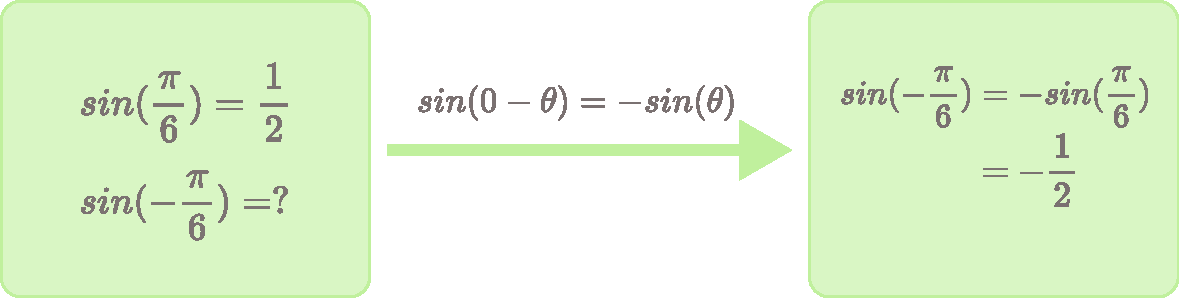
\includegraphics[width=0.75\linewidth]{assets/prelude/symbolic-transform.pdf}
    % \vspace{-10pt}
\end{figure*}

\setlength{\columnsep}{1em}
\setlength{\intextsep}{0em}
\begin{wrapfigure}{r}{.23\textwidth}
\vspace{-10pt}
  \begin{center}
    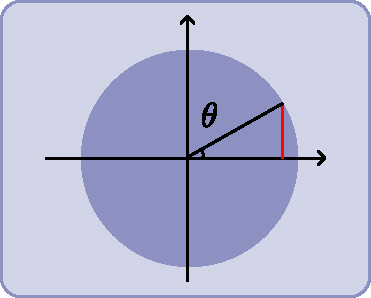
\includegraphics[width=0.23\textwidth]{assets/prelude/unit-circle.pdf}
  \end{center}
\end{wrapfigure}

A useful visual representation of this concept is the unit circle: on a Cartesian plane with a circle of radius $1$ centered at the origin, concrete values of trig functions are represented visually and rules are implicitly encoded as geometric transformations. For instance, the value of $sin(\theta)$ is the y-coordinate of a point on the circle, where the ray from the origin to the point forms angle $\theta$ with the x-axis.

To derive the identity rule visually, one only needs to note that $-\theta$ is a reflection about the x-axis, and observe that the y-coordinate is now a negative number. Instead of having to memorize a big set of rules, one can reduce this problem to a simple operation on the visual representation of a unit circle.

\vspace{10pt}
\begin{figure*}[h]
    \centering
    \includegraphics[width=0.70\linewidth]{assets/prelude/visual-transform.pdf}
    % \vspace{-10pt}
\end{figure*}

By translating the symbols to a visual representation, a unit circle, a student completely bypasses the tedious memorization of trig identities. While this is a much more retainable and robust representation for students, are we teaching representations like this to students? What does it take for students to internalize it? 

\chapter{Introduction}

``Mental pictures'' and ``visual intuition'' capture how people make sense of abstract concepts and see solutions to hard problems in a visual way. Hadamard described numerous examples of mathematicians doing exactly this in \emph{The Mathematician's Mind}~\cite{Hadamard1997a}, later summarized by Alan Kay~\cite{doingWithImages}:

\begin{quote}
Jacques Hadamard, the famous French mathematician, in the late stages of his life, decided to poll his 99 buddies, who made up together the 100 great mathematicians and physicists on the earth, and he asked them, ``How do you do your thing?'' They were all personal friends of his, so they wrote back depositions. Only a few, out of the hundred, claimed to use mathematical symbology at all. Quite a surprise. All of them said they did it mostly in imagery or figurative terms.
\end{quote}

Learning research suggests that visual representations of knowledge are powerful tools for thought. Visual representations like diagrams enable more robust learning \cite{multimediaLearning} and abstract and flexible problem solving~\cite{Koedinger1990a, pictureAlgebra, DiagramsThousandWords}. Importantly, when people work with visuals, they build better conceptual understanding and more flexible mental models that go beyond memorized procedures~\cite{multipleReps}.

\setlength{\columnsep}{1em}
\setlength{\intextsep}{0em}
\begin{wrapfigure}{r}{.45\textwidth}
\vspace{-10pt}
  \begin{center}
    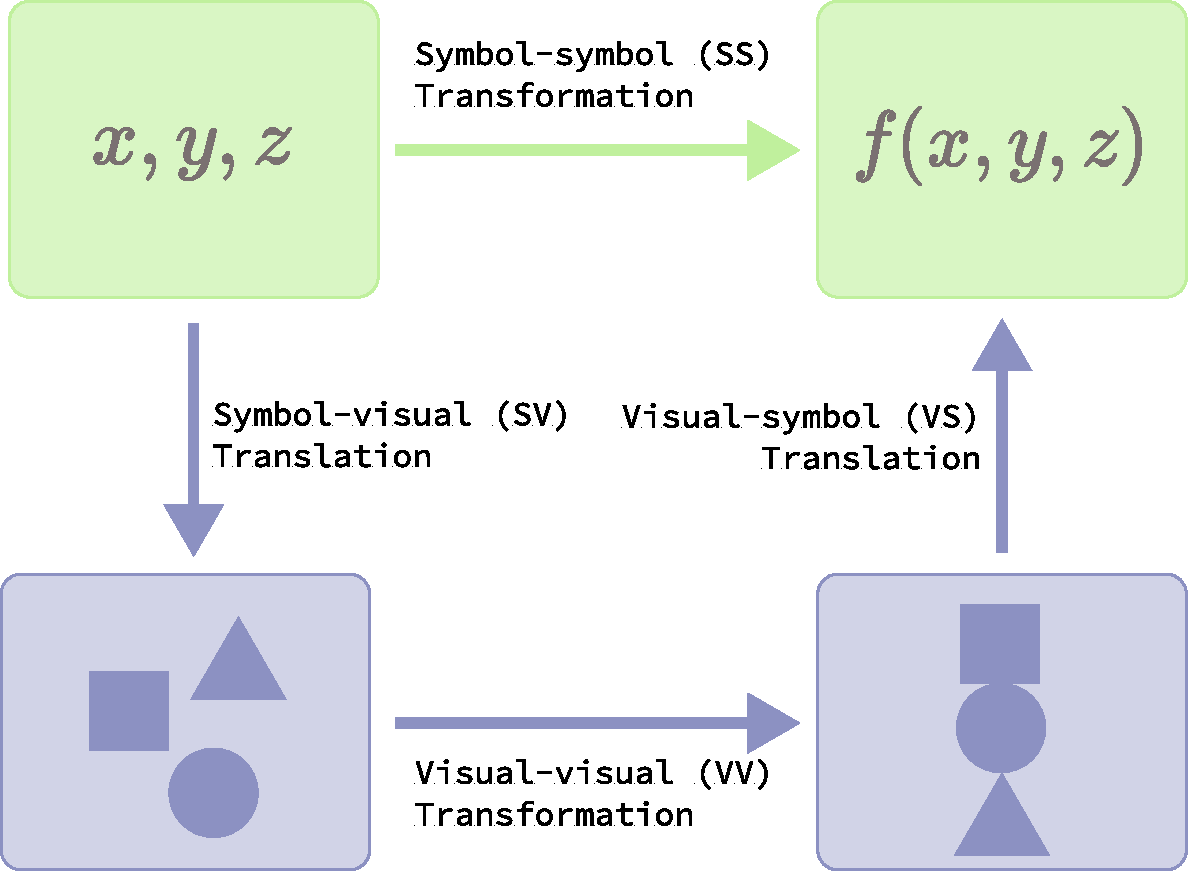
\includegraphics[width=0.45\textwidth]{assets/chapter-1/grounding-rectangle.pdf}
  \end{center}
\end{wrapfigure}

Let me use a diagram to capture this: the \textbf{grounding rectangle} represents two pathways to learning and problem solving: One can perform symbol-to-symbol transformations (SS, or “symbol pushing”) or through an \textcolor[HTML]{8C91C2}{alternative diagrammatic pathway}: a symbol-to-diagram translation (SV), a diagram-to-diagram transformation (VV), and finally a diagram-to-symbol translation (VS).

Research on expertise development suggests a need for substantial exposure involving repetition in varied contexts or deliberate practice \cite{deliberatePractice} to acquire the perceptual chunks \cite{chunkingModels, perceptualLearningExpertise} that support accurate interpretation and use of visual representations~\cite{Koedinger1990a}. Through enough practice, learning the two paths in the grounding rectangle can produce better, more robust memory \cite{dualCoding}, learning~\cite{multipleReps, multimediaLearning, cotraining}, and future reasoning, both in providing flexibility and in supporting error recovery \cite{groundedAndAbstractReps}.

In reality, there seems to be an over-abundance of symbolic practice, continuing Kay's train of thought:

\begin{quote}
    The sad part of the diagram is that every child in the United States is taught math and physics through this [symbolic] channel. The channel that almost no adult creative mathematician or physicist uses to do it... They use this channel to communicate, but not to do their thing.
\end{quote}

Diagrammatic practice is rare due to the significant cost of authoring diagrammatic problems. Existing diagramming tools often require hours of low-level tweaking of geometric primitives and do not capture the core task of diagramming: representing ideas visually. In other words, these tools lack \emph{representational salience}. As a result, the diagrams created by existing tools don't have semantics, as they are merely a collection of pixels and geometric blobs.  

In prior work, colleagues and I built \Penrose, a diagramming platform that explicitly encodes visual representations in domain-specific languages (DSLs)~\cite{penrose}. In this thesis proposal, I argue that this explicit encoding can be leveraged to (1) reduce the programming effort of producing diagrammatic problems at scale and (2) simplify the workflow of authoring interactive diagrams. The resulting diagrams also carry rich semantics, and I propose to use them to (3) provide useful, automated feedback to students. My thesis statement summarizes the above:

\vspace{10pt}
\boxtext{
\textbf{Encoding visual representations in diagramming tools simplifies programming of interactive visual activities that provide students with automated feedback at scale.}
}
\vspace{10pt}

The expected contributions of this work are:

\begin{enumerate}
    \item \emph{Need-finding studies} on challenges authors face.
    \item \emph{A platform of tools} based on the visual encoding of \Penrose for mass-production of diagrams (\cref{chp:edgeworth}) and rapid authoring of interactive diagrams (\cref{chp:ipenrose}).
    \item \emph{A theoretical framework} of the grounding rectangle, which guides the design of tools presented in this proposal.
\end{enumerate}

\begin{proposed}
\textbf{Note.} This proposal contains a mix of completed, in-progress, and proposed projects. In the rest of this document, proposed work will be marked in orange on the left margin. 
\end{proposed}

\chapter{Understanding the diagramming process and encoding visual representations}
\label{chp:diagrammingAndPenrose}

Before diving into the educational context, it's important to understand why creating diagrams is hard in the first place. This chapter discusses an interview study on how domain experts including educators use diagramming tools~\cite{naturalDiagramming}, and briefly shows how this study informs the design of \Penrose, the technical basis for tools presented in this proposal. 

\section{How domain experts create diagrams and implications for tool design}
\label{sec:naturalDiagramming}

Existing diagramming tools stand in tension between: a) General-purpose drawing tools such as Illustrator and Figma that offer simple pen-and-canvas or box-and-arrow metaphors, but are viscous~\cite{cognitiveDimensions}---users must constantly commit to exact positions, sizes, and styling of shapes. b) Dedicated diagramming tools such as Lucidchart and Gliffy that allow rapid changes, but rely heavily on templates, limiting diagrammers to a fixed set of visual representations. This relatively limited support for diagramming in tools is in part because the process of diagramming is poorly understood. For instance, how do diagrammers utilize the strengths and cope with the limitations of their tools? Which tools are chosen for what purposes?  Such a detailed understanding of the process can help design interactive tools to support diagramming.

I conducted interviews with 18 domain experts from a wide variety of disciplines such as math, computer science, architecture, and education. The interviews reveal that diagrammers have diverse interactions with visual representations in both physical sketches and digital tools, including finding, creating, storing, and reusing representations. 

One implication of our results is the opportunity to design tools informed by the processes of diagramming, and practices that domain experts already use, making digital diagramming more intuitive and efficient. Here are four key opportunities for natural~\cite{naturalProgramming} diagramming tools that allow diagrammers to express their ideas visually the same way they think about them:

\begin{itemize} 
    \item \textit{Exploration support}: supporting exploratory behaviors such as undo and backtracking during both abstract-level, breath-first exploration of the design space and low-level refinements of visual details.
    \item \textit{Representation salience}: allowing explicit creation and management of visual representations, \ie, the \emph{mappings} from domain constructs to shapes instead of geometric primitives themselves.
    \item \textit{Live engagement}: providing diagrammers with the sense of agency by designing for liveness and directness of the diagramming experience. 
    \item \textit{Vocabulary correspondence}: enabling diagrammers to interact with their diagrams using vocabularies that is conventional in their domain.
\end{itemize}

\section{The design of \Penrose}
\label{sec:penrose}

Informed by the results from the interview study, colleagues and I have developed \Penrose, a language-based diagramming platform~\cite{penrose}. The core \Penrose system addresses \textbf{representation salience} and \textbf{vocabulary correspondence}: it has first-class support for creating and reusing visual representations and translates familiar math-like notation into one or more possible visual representations. To accomplish this, \Penrose decomposes the concerns of diagramming into two domain-specific languages (DSLs) with distinct purposes: \colorbox[HTML]{E7F3E7}{\Substance} contains the mathematical content in math notation. \colorbox[HTML]{DDDEED}{\Style} explicitly specifies mappings from mathematical objects to visual icons. 

\setlength{\columnsep}{1em}
\setlength{\intextsep}{0em}
\begin{wrapfigure}{r}{.45\textwidth}
\vspace{-10pt}
  \begin{center}
    \includegraphics[width=0.45\textwidth]{assets/chapter-2/penrose-trio.pdf}
  \end{center}
\end{wrapfigure}

Instead of a limited focus on one specific domain (as in GraphViz~\cite{graphviz} for graph theory or GroupExplorer~\footnote{\url{https://github.com/nathancarter/group-explorer}} for group theory), \Penrose is extensible to user-defined domains of diagramming. Both \Substance and \Style are parametrized by a \colorbox[HTML]{DBDBDB}{\Domain} schema that defines all possible objects (\eg, \sub{Set}) and relations (\eg, \sub{IsSubset}) in a particular domain, which can be used by associated \Substance and \Style programs. In addition to user-extensibility, a formally encoded domain also enables automatic generation of \Penrose diagrams. 

\Penrose compiles a \textbf{trio} of \Domain, \Substance, and \Style into a constrained optimization problem defined by a set of graphical constraints (\eg, arrows that represent vectors should start from the origin). The optimization problem is in standard form, \ie, minimization of an objective function subject to equality and inequality constraints~\cite{convexOptimization}. Such problems may be solved with many standard methods. \Penrose currently uses an exterior point method~\cite{exteriorPoint} that starts with an infeasible point and pushes it toward a feasible configuration via progressively stiffer penalty functions---mirroring a process often used by hand.

The design of \Penrose is driven by the design goals of reuse and scalability, and therefore is suitable for large-scale generation of visual content. The system is scalable and reusable in several dimensions:
    
% \setlength{\columnsep}{1em}
% \setlength{\intextsep}{0em}
% \begin{wrapfigure}{r}{.45\textwidth}
% \vspace{-10pt}
%   \begin{center}
%     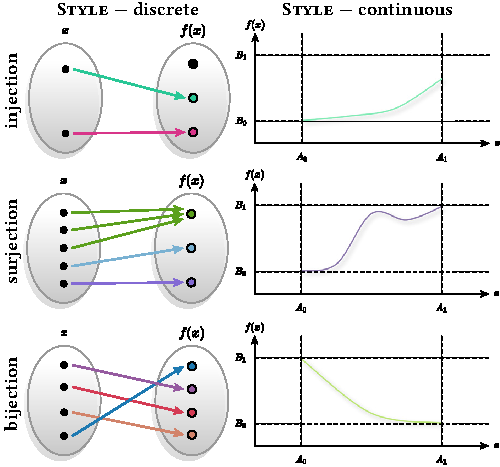
\includegraphics[width=0.45\textwidth]{assets/chapter-2/func-continuous-discrete-vert.pdf}
%   \end{center}
% \end{wrapfigure}

\vspace{1em}
\begin{figure}[h]
\begin{minipage}[b]{0.48\linewidth}
$\bullet$ The optimization problem produced by \Penrose often has multiple solutions, and each point in the solution space corresponds to an alternative diagram. No program changes are required to generate these alternatives.
    \vspace{3pt}

$\bullet$ For a visual representation encoded by a \Style program, a wide range of notations (\ie, \Substance programs) can be visualized without any changes to \Style. In the figure on the left, a single discrete \Style program is used to visualize three \Substance programs that describe injective, surjective, and bijective functions.
    \vspace{3pt}

$\bullet$ Conversely, multiple \Style{} programs can be applied to the same \Substance{} program, generating alternative visual representations of the same underlying entities. The \Substance programs in the figure are also visualized by an alternative continuous \Style.
\end{minipage}
\hfill
\begin{minipage}[b]{0.5\linewidth}
    \centering
    \includegraphics[width=\textwidth]{assets/chapter-2/injection-surjection-bijection.pdf}
\end{minipage}
\end{figure}
    
With the extensible design, \Penrose can automatically generate diagrams from many different domains using familiar syntax. \Penrose-generated geometry, real analysis, ray-tracing, set theory, and algebra are shown below.

\vspace{10pt}
\includegraphics[width=0.95\linewidth]{assets/chapter-2/gallery.pdf}




% \chapter{From encoding to semantics-preserving interactivity}
% \label{chp:ipenrose}

% Diagrams live in the context of surrounding text, overlaid annotations, and human gestures. The web opens up opportunities for even richer in-context interaction. In education, though students spend more time on digital platforms, they often see diagrams that are presented exactly as before: blurry, static, and ornamental. In addition to their values as an external, static representation of knowledge, diagrams are also beneficial when people learn \emph{with}, instead of \emph{from} them~\cite{learningWithRepresentations}.  Prior work shows interacting with visual representations has unique benefits to learning \cite{drawingToLearn, VisualexplanationsImprovesLearning}. In contrast with a static diagram, \textbf{a semantics-preserving interactive diagram allows students to rapidly explore alternatives, understand the underlying rules of a visual representation, and receive instant feedback on their actions.} Meaningful interaction with diagrams helps students move from passive recognition to active synthesis of visual representations~\cite{bloomRevised}.

% Sadly, interactive diagrams are scarce in the wild. Most interactive documents require authors to be proficient in general-purpose programming and have decent knowledge in handling low-level events like mouse down/up, hover, etc. As a result, a simple interactive diagram often takes up 100s of lines-of-code and can be hard to debug~\cite{callbackSpaghetti, usabilityInteractionTools}. Additionally, because interactive diagrams change a lot, authors often need to reason about a collection of diagrams, making the task even harder.

% \Penrose and \Edgeworth elevate the semantics of diagrams from low-level primitives to mathematically meaningful notations. Specifically, \Penrose encodes both the translational semantics of how notations are translated to diagrams, and the visual semantics of how shape primitives relate to each other expressed as constraints. By exploiting both, we can automatically support semantics-preserving interactive diagrams. In this section, I investigate how to build interactive diagram activities that are automatically derived from \Penrose diagrams and easily created without extensive programming efforts. In short, I propose to \textbf{(1) simplify programming interactive diagrams and (2) provide students with rich, automated feedback by leveraging the encoding of visual representations}. 

% \section{Motivating example}
% \label{sec:ipenrose-example}

% Consider the first diagram in a popular explorable explanation piece ''Eigenvectors and Eigenvalues Explained Visually~\footnote{\url{https://setosa.io/ev/eigenvectors-and-eigenvalues/}}.''  The diagram is one of a series of interactive diagrams showing the visual properties of eigenvalues and eigenvectors: it shows a visual interpretation of matrices as linear transformations: matrix $A$ with columns $a_1$ and $a_2$ transforms $v$ to $Av$. In the diagram, $a_1$, $a_2$ and $v$ are all draggable. 

% \begin{figure}[h]
%     \centering
%     \includegraphics[width=0.8\linewidth]{assets/chapter-4/eigen-visually.pdf}
% \end{figure}

% Seeing what varies and what doesn't is an important form of \emph{feedback} that fosters conceptual understanding. The reader gains an initial understanding of how columns of $A$ impact $Av$’s value through interacting with the diagram: dragging any of $a_1$, $a_2$ and $v$ affects the position of $Av$. 

% In the original code repository~\footnote{\url{https://github.com/vicapow/explained-visually/tree/master/client/explanations/eigenvectors-and-eigenvalues}}, the authors wrote about a hundred lines of JavaScript with D3.js to make the first diagram. Although D3.js and Angular already provide significant support, it's still a lot of work to handle mouse down/up/hover events, and to keep track of intermediate values during dragging. 

% To reproduce this diagram in \Penrose, one can write a simple \Substance program in the linear algebra domain~\cite[Section 5.4]{penrose}. 

% \begin{figure}[h]
%     \centering
%     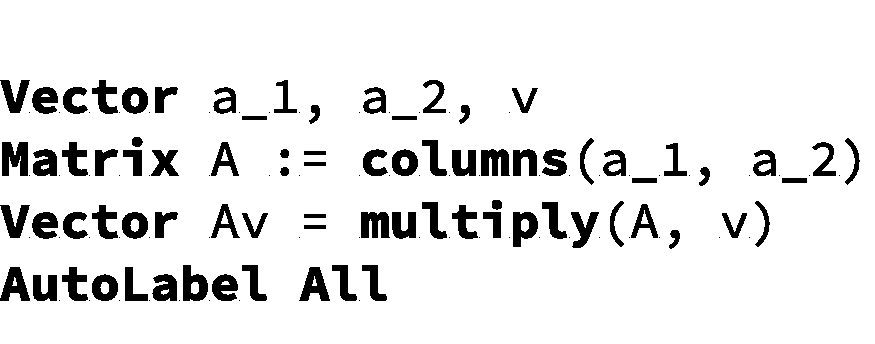
\includegraphics[width=0.4\linewidth]{assets/chapter-4/eigen-substance.pdf}
% \end{figure}

% With the core system, the trio generates a static SVG diagram. Under the hood, every \sub{Vector} is represented visually as an arrow starting at the origin ($a_1$, $a_2$), or a single point ($v$). They are all degrees of freedom (DOF) in the optimization problem. In other words, both the x and y-components of the arrow-end of  $a_1$, $a_2$, and the point representing $v$ are free to move on the canvas. Following the original design of the explorable, the system surfaces the DOFs as draggable points. Whenever the user drags the end of one of the arrows, the optimizer takes the new position as a part of the final solution, and solves the rest of the optimization problem. Effectively, by using this simple and generalizable strategy, which I will discuss in the following sections, the system can reproduce the interactive design using the \Penrose trio for a static diagram \emph{without a single line of code added}.

% \section{Semantics-preserving interactivity as feedback}
% \label{sec:semantic-drag}

% \begin{proposed}
% \cref{sec:ipenrose-example} is an example of a set of interactive behaviors that can be automatically derived from a \Penrose trio without any additional programming.  Specifically, the example leverages how \Penrose encodes visual semantics: \Penrose compiles a program trio to computational and optimization graphs with degrees-of-freedom (DOF)~\cite[Section 4.1.2-3]{penrose}. Degrees-of-freedom determine a diagram instance in \Penrose. They are ``free'' variables within the computational graph and non-constant root nodes in the optimization graph. DOFs are the key to generate a family of diagrams: by manipulating DOFs, the optimizer solves for different diagrams that satisfy the constraint set defined by the trio. In other words, DOFs are a concise representation for interaction. In this section, I use \emph{dragging} as a case study and show a few ways of manipulating the DOFs in a semantics-preserving manner. 

% As a reasonable default, the system can find positional properties in the DOFs and make them draggable. In \cref{sec:ipenrose-example}, the relevant \Style blocks define a simple computational graph for the \Substance program, where \sty{a_1.data}, \sty{a_2 .data}, and \sty{v.data} are DOFs. \cref{fig:eigen-comp-graph} shows the graph for \sty{a_1}’s properties. To accomplish the interactivity in the example, the system can analyze the computational graph to find DOFs and their aliases, \ie, child nodes that are assigned values of the DOFs. For instance, \sty{a_1.data} is a DOF and \sty{a_1.icon.end} references \sty{a_1.data}. In contrast, \sty{Av.end} is not made draggable because it's not a DOF nor an alias in the computational graph: its value is computed by \sty{matmul(a_1.data, a_2.data)}.

% \vspace{10pt}
% \begin{figure}[h]
%     \centering
%     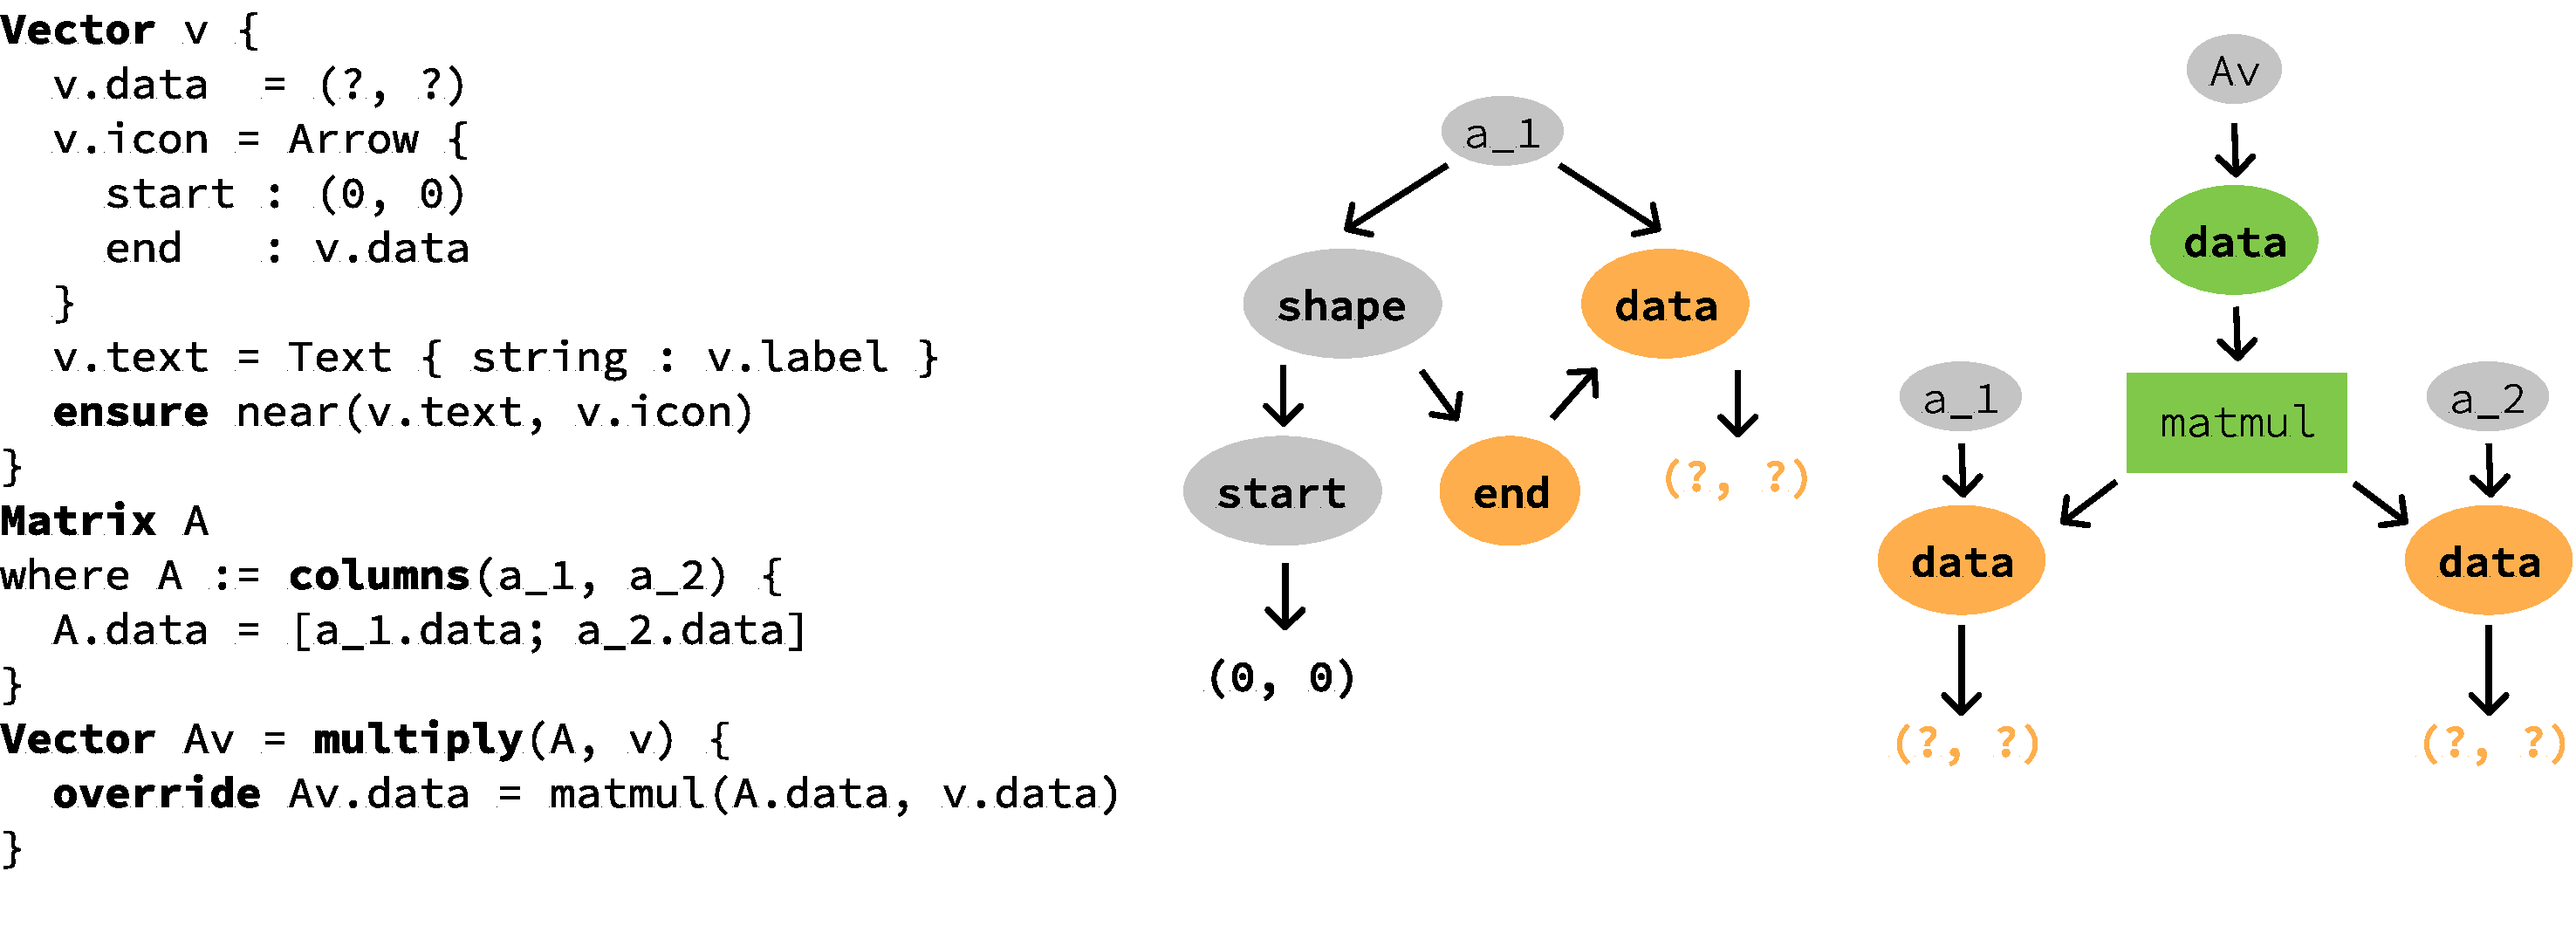
\includegraphics[width=\linewidth]{assets/chapter-4/eigen-comp-graph.pdf}
%     \vspace{-30pt}
%     \caption{\textbf{Left}: relevant blocks in the linear algebra \Style program for \cref{sec:ipenrose-example}. \textbf{Right}: computational graphs for \texttt{a\_1} and \texttt{Av}, where the \texttt{data} field for the former is optimized and that for the latter is computed.}
%     \label{fig:eigen-comp-graph}
% \end{figure}
% \vspace{10pt}

% Once exposed as draggable properties, the user can now change the values of positional DOFs by dragging shapes around. However, since their interaction is situated in an optimization problem, it's important to discuss how an optimizer influences this interaction and manipulates the rest of the diagram in a semantics-preserving way. In \cref{sec:ipenrose-example}, dragging \sty{a_1.icon.end} and \sty{a_2.icon.end} works as intended because they are independent from each other: they don't participate in the same constraints in the computational graph. However, this is not the right interaction for DOFs that participate in the same constraints, which is often the case. In this section, I give two example optimization strategies for supporting semantics-preserving drag.    
% \subsection{Follow the cursor}
% \label{sec:follow-the-cursor}

% \vspace{10pt}
% \begin{figure}[h]
%     \centering
%     \includegraphics[width=0.8\linewidth]{assets/chapter-4/drag-expected.pdf}
%     \caption{Dragging a subset, $B$, in a Venn diagram in an intuitive and semantics-preserving way, where $B$ is always under the cursor and $B \subset A$ is always held true.}
%     \label{fig:drag-expected}
% \end{figure}
% \vspace{10pt}

% Consider the example in \cref{fig:drag-expected}, which shows a simple Venn diagram of sets $A$ and $B$ where $B \subset A$. The underlying rule of this visual representation is that a subset is always visually contained in the superset. An interactive diagram should clearly reveal this rule by keeping this containment relationship true at all times. For instance, if a student drags $B$ to the right, the diagram should change such that $A$ still contains $B$. Importantly, the interaction should be natural, and also make the feedback very clear: as the student is dragging $B$, $B$ must stay under the cursor, and the rest of the diagram should incrementally move with $B$ to maintain the containment relationship.

% Unfortunately, when using the current \Penrose optimizer, dragging either $A$ or $B$  yields counterintuitive results: the optimizer changes arbitrary properties, including the manipulated ones. This is because it optimizes all DOFs simultaneously. In \cref{fig:drag-default}, it moves both $A$ and $B$ to satisfy the containment constraint.  This behavior adds noise to the feedback, and may confuse the student.

% \vspace{10pt}
% \begin{figure}[h]
%     \centering
%     \includegraphics[width=0.75\linewidth]{assets/chapter-4/drag-default.pdf}
%     \caption{Dragging a subset, $B$, in a Venn diagram in semantics-preserving but counterintuitive way, where $B \subset A$ held true but the shapes appear in random locations.}
%     \label{fig:drag-default}
% \end{figure}
% \vspace{10pt}

% To enable intuitive interactivity, the system can analyze the computational graph again to derive the right behavior. We can achieve this behavior by ``locking'' the DOFs, treating them as constants in the optimizer. Specifically, when a student manipulates DOFs or its aliases, the system locks these DOFs and optimizes the rest as usual. When the student interacts with an object (\ie, dragging to change \sty{x} and \sty{y} of a \sty{Circle}), the system yields the control to the student completely and locks the manipulated properties during optimization. The visual effect is that all other parts of the diagram ``follow'' the student interaction. 

% \subsection{Freeze the world}
% \label{sec:freeze-the-world}

% Locking the manipulated property is not the only way to maintain the visual semantics. Instead of limiting the optimizer, we could also limit the interaction so they see the effect of changing one or multiple shape properties under constraints. When the student interacts with a shape, the optimizer keeps all other properties locked and continuously uses the energy function to “guide” the student. The techniques involved are different from \cref{sec:follow-the-cursor}. In this case, the student is playing the role of the optimizer, \ie, changing DOFs, while the optimizer only sends feedback to make sure the interaction is semantic. The visual effect is a constrained interaction where the student can only make semantically-valid moves. 

% \vspace{10pt}
% \begin{figure}[h]
%     \centering
%     \includegraphics[width=0.75\linewidth]{assets/chapter-4/unit-circle-drag.pdf}
%     \caption{The behavior of dragging a point along the unit circle depends on the optimization strategy. \textbf{Left}: ``Follow the cursor'' shifts the entire diagram to follow the point and doesn't correspond to the mathematical semantics. \textbf{Right}: ``Freeze the world'' should be the correct optimization strategy, where the point only moves along the circle, and nothing else changes in the diagram.}
%     \label{fig:unit-circle-drag}
% \end{figure}
% \vspace{10pt}


% For instance, \cref{fig:unit-circle-drag} shows a diagram of the unit circle. A natural interaction is to drag the point along the unit circle to see how the values of trig functions change. In this case, the red line shows the value of $sin$. If the optimizer naively follows the cursor, \cref{fig:unit-circle-drag} (right) would be the result, where the rest of the diagram is translated to stay in a valid layout. Instead, it's much more desirable to ``freeze the world'' and constrain the student input within the feasible region—--along the unit circle (\cref{fig:unit-circle-drag} left).

% Together, these two strategies cover a wide range of drag behaviors that are traditionally difficult and time-consuming to implement. Note that these two strategies are not necessarily mutually exclusive. In fact, the system may have a set of default rules for or let the author specify the strategy on a per-DOF basis. For instance, an instructor might apply ``freeze the world'' to show students the valid positions of a component in a diagram, while applying ``follow the cursor'' to the rest of the components to show alternative layouts of the diagram. 


% \vspace{10pt}
% \noindent\textbf{Encoding optimization strategies.} If the author wants to control the optimization strategy, they will need an encoding to do so. Because \Style already has language constructs for matching on shapes, a \Style language extension may be suitable for specifying static strategies per shape, \eg, a shape should always follow the cursor when dragged. However, the current design of \Style may not be suitable for deciding strategies dynamically if needed, \eg, a shape follows the cursor in a certain region of the diagram, and freezes the world on the boundary. 
% \end{proposed}

% \section{Highlighting and annotation as feedback}
% \label{sec:highlight-and-annotate}

% \begin{proposed}

% As demonstrated in \cref{chp:edgeworth}, diagram understanding is a vital step towards representational fluency. A significant part of diagram understanding maps to learning the translational semantics of a diagram, \ie, which shape represents what math object. While \Edgeworth helps students practice the mapping between a particular visual representation and symbols, I propose to \textbf{provide on-demand, inter-representational feedback by utilizing the translational semantics of a \Penrose trio}. 

% \subsection{Inter-representational highlighting}

% Students' exposure to visual representations is often limited by traditional media like textbooks and in-person lectures. The mapping between symbolic and visual representations is often scarcely presented via prose, gesture, and carefully designed worked examples. Web-based materials show a much more pervasive use of on-demand highlighting to build up inter-representational connections. However, there’s also a non-trivial authoring burden to meticulously annotate the HTML document and the diagram with CSS classes:

% \vspace{10pt}
% \begin{figure}[h]
%     \centering
%     \includegraphics[width=\linewidth]{assets/chapter-4/euclid-highlight.pdf}
%     % \label{fig:euclid-highlight}
% \end{figure}
% \vspace{10pt}

% If an online textbook or website uses diagrams generated by \Penrose, the author may leverage the translational semantics to automatically provide on-demand highlights. For instance, suppose an author writes an visual explanation in markdown with interleaving \Substance symbols in the prose. The system can automatically generate diagrams by extracting the \Substance symbols and provide highlights for all subsequent references to the same symbols. Since \Penrose can generate alternative diagrams in the same visual presentations, the highlighting can also provide contrasting cases of a particular entity across diagram instances.

% \vspace{10pt}
% \begin{figure}[h]
%     \centering
%     \includegraphics[width=\linewidth]{assets/chapter-4/markup-highlight.pdf}
% \end{figure}
% \vspace{10pt}

% Building connections among multiple visual representations also improve learning~\cite{multipleReps}. Because a \Penrose trio is representationally salient, one can swap among alternative \Style programs to get diagrams that visualize the same symbols. Because the \Substance program stays the same, the same strategy also works for highlighting diagram parts across multiple visual representations.

% \vspace{10pt}
% \begin{figure}[h]
%     \centering
%     \includegraphics[width=0.9\linewidth]{assets/chapter-4/multirep-highlight.pdf}
% \end{figure}
% \vspace{10pt}

% \subsection{Documentation and program slices as tooltips} 

% \vspace{10pt}
% \begin{figure}[h]
%     \centering
%     \includegraphics[width=\linewidth]{assets/chapter-4/docs-tooltips.pdf}
% \end{figure}
% \vspace{10pt}

% In technical documents, symbols and acronyms are often defined once and used everywhere else. To help readers understand them, tools like ScholarPhi and Nota~\cite{scholarPhi, nota} use tooltips to aid readers. In real world publications, authors augment math equations for better readability, too. Diagrams use even more symbolism and can be hard to understand. We propose a lightweight markup language in the form of \Substance documentation for authoring simple \emph{diagram augmentation}. Similar to Idyll~\cite{idyll}, the markup language has a markdown-like syntax, but allows splices of \Substance variables and runtime values. In the frontend, we analyze the \Substance values in each snippet, and trace all related snippets based on variable references. For instance, the snippet about $Av$ refers to both $A$ and $v$, so they appear on the tooltip stack.

% The translational semantics also involve how \Domain, \Substance, and \Style programs relate to each other. Therefore, \Style and \Domain can also be valuable sources of feedback: the \Style program encodes the visual semantics, and the \Domain program captures the grammar of notations. A slice of a \Penrose trio traces the origin of a graphical primitive to the \Domain, \Substance, \Style programs. For instance, without any authoring burden, the system can display slices of the program trio based on object selection. Alternatively, the proposed markup language may be extended to \Domain and \Style, and the system can render inline documentations in all three languages.

% \vspace{10pt}
% \begin{figure}[h]
%     \centering
%     \includegraphics[width=0.75\linewidth]{assets/chapter-4/slices.pdf}
% \end{figure}
% \vspace{10pt}
% \end{proposed}

% \section{Evaluation}

% \begin{proposed}
% To evaluate the discussed interactive techniques, I plan to conduct comparative case studies between feature-full modern JavaScript libraries (e.g. D3.js) and \Penrose. Research questions for this study include:
% \begin{itemize}
%     \item Does the \Penrose-based system simply programming interactive diagrams?
%     \item Are the interactive features comparable to the hand-written examples? 
%     \item How expressive is our grammar of interactivity?
%     \item When does the approach break down?
% \end{itemize}

% In general, I expect that our system can cover common, important interactive features with significantly less manual effort. In the studies, I plan to collect both quantitative (\eg, lines-of-code, time taken) and qualitative data about authoring interactive diagrams using JS library versus our system. Currently, the candidate pool of examples include:

% \begin{itemize}
% \item Worked examples and explorable explanations:
%     \begin{itemize}
%         \item A Gentle Introduction to Graph Neural Networks: \url{https://distill.pub/2021/gnn-intro/}
%         \item Explained visually: \url{https://setosa.io/ev/}
%         \item Explorable explanations: \url{https://explorabl.es/}
%         \item Gallery of concept visualization: \url{https://conceptviz.github.io/}
%     \end{itemize}
% \item Online textbooks and curricula:
%     \begin{itemize}
%         \item Seeing theory: \url{https://seeing-theory.brown.edu/}
%         \item Immersive math: \url{http://immersivemath.com/ila/index.html}
%         \item Mathigon: \url{https://mathigon.org/}
%         \item Physically-based rendering: \url{https://pbr-book.org/}
%         \item Brilliant: \url{https://brilliant.org/}
%     \end{itemize}
% \end{itemize}
% \end{proposed}

% \section{Related work}

% \subsection{Grammars for interactivity}

% Pioneered by the grammar of graphics~\cite{grammarOfGraphics}, researchers in data visualization developed a rich set of tools based on an explicit encoding of the mapping from data to visual primitives~\cite{d3, vega, vegalite}. Notably, Vega-Lite~\cite{vegalite} is a grammar for interactive data visualization. One key to the Vega-Lite grammar is ``selection,'' because the underlying data doesn't change during interaction. In diagramming, this assumption is not always true. The basic building blocks are mostly ``manipulation'' of shapes in relation with the underlying representation. \citet{datavizCriticalReflection} give an extensive review of data visualization authoring tools, including those that support interactivity.

% In addition, the information/data visualization literature also contributed taxonomies and conceptual frameworks of interactivity. For instance, \citet{infovizInteractionFramework} propose 7 general categories of interactive techniques in information visualization: Select, Explore, Reconfigure, Encode, Abstract/Elaborate, Filter, and Connect. Similarly, \citet{interactiveDynamicsTaxonomy} describe a taxonomy of interactive dynamics for visual analysis, which was presented as a list of verbs, too. These frameworks and taxonomies are useful to build upon. Again, the high-level concepts involved for interactive diagrams can change significantly from them because of the differences between diagrams and data/information visualization~\cite{naturalDiagramming}, 

% \subsection{Constraint-based interactivity}

% In the HCI literature, there’s a long line of work on authoring interactive user interfaces using constraints. For instance, Garnet~\cite{garnet} and Amulet~\cite{amulet} use dataflow constraints to build highly interactive UIs. In these systems, the author declaratively specifies constraints on the relationship among graphical elements in terms of data dependencies (i.e. $D = f(l_1, l_2, \dots, l_n)$, and the interactivity is handled by a constraint solver at runtime. Thinglab~\cite{thinglab} supports simultaneous equations for building simulations. At its core, the \Penrose system is a combination of dataflow constraints (computations) and simultaneous equations (constraints and objectives). Therefore, many of the techniques from this line of work may apply to supporting interactivity in \Penrose, such as efficient incremental constraint solving~\cite{deltablue}.


% \chapter{\Edgeworth project plan}

% To address the committee feedback from the thesis proposal presentation, this appendix to the proposal document elaborates on \cref{chp:edgeworth}. This elaboration comes in acknowledgment that the committee sees the goals in \cref{chp:ipenrose} as optional.  In this appendix, I summarize the proposed elaboration on \cref{chp:edgeworth}, describe the research hypotheses, and outline the evaluation plan for validating them. The intention of this appendix is to specify all of the required work in the dissertation.

% In the proposal document, \cref{chp:edgeworth} describes the following completed work on \Edgeworth:

% \begin{itemize}
%     \item Formative interviews with 6 educational content authors
%     \item Design and implementation of mutation operators in the \Edgeworth mutator
%     \item A prototype of the \Edgeworth mutator with a configuration-based workflow
%     \item Preliminary evaluation of the prototype by re-creating problems in a geometry textbook
% \end{itemize}

\chapter{\Edgeworth: diagrammatic problem authoring at scale}
\label{chp:edgeworth}

\begin{figure}[h]
    \centering
    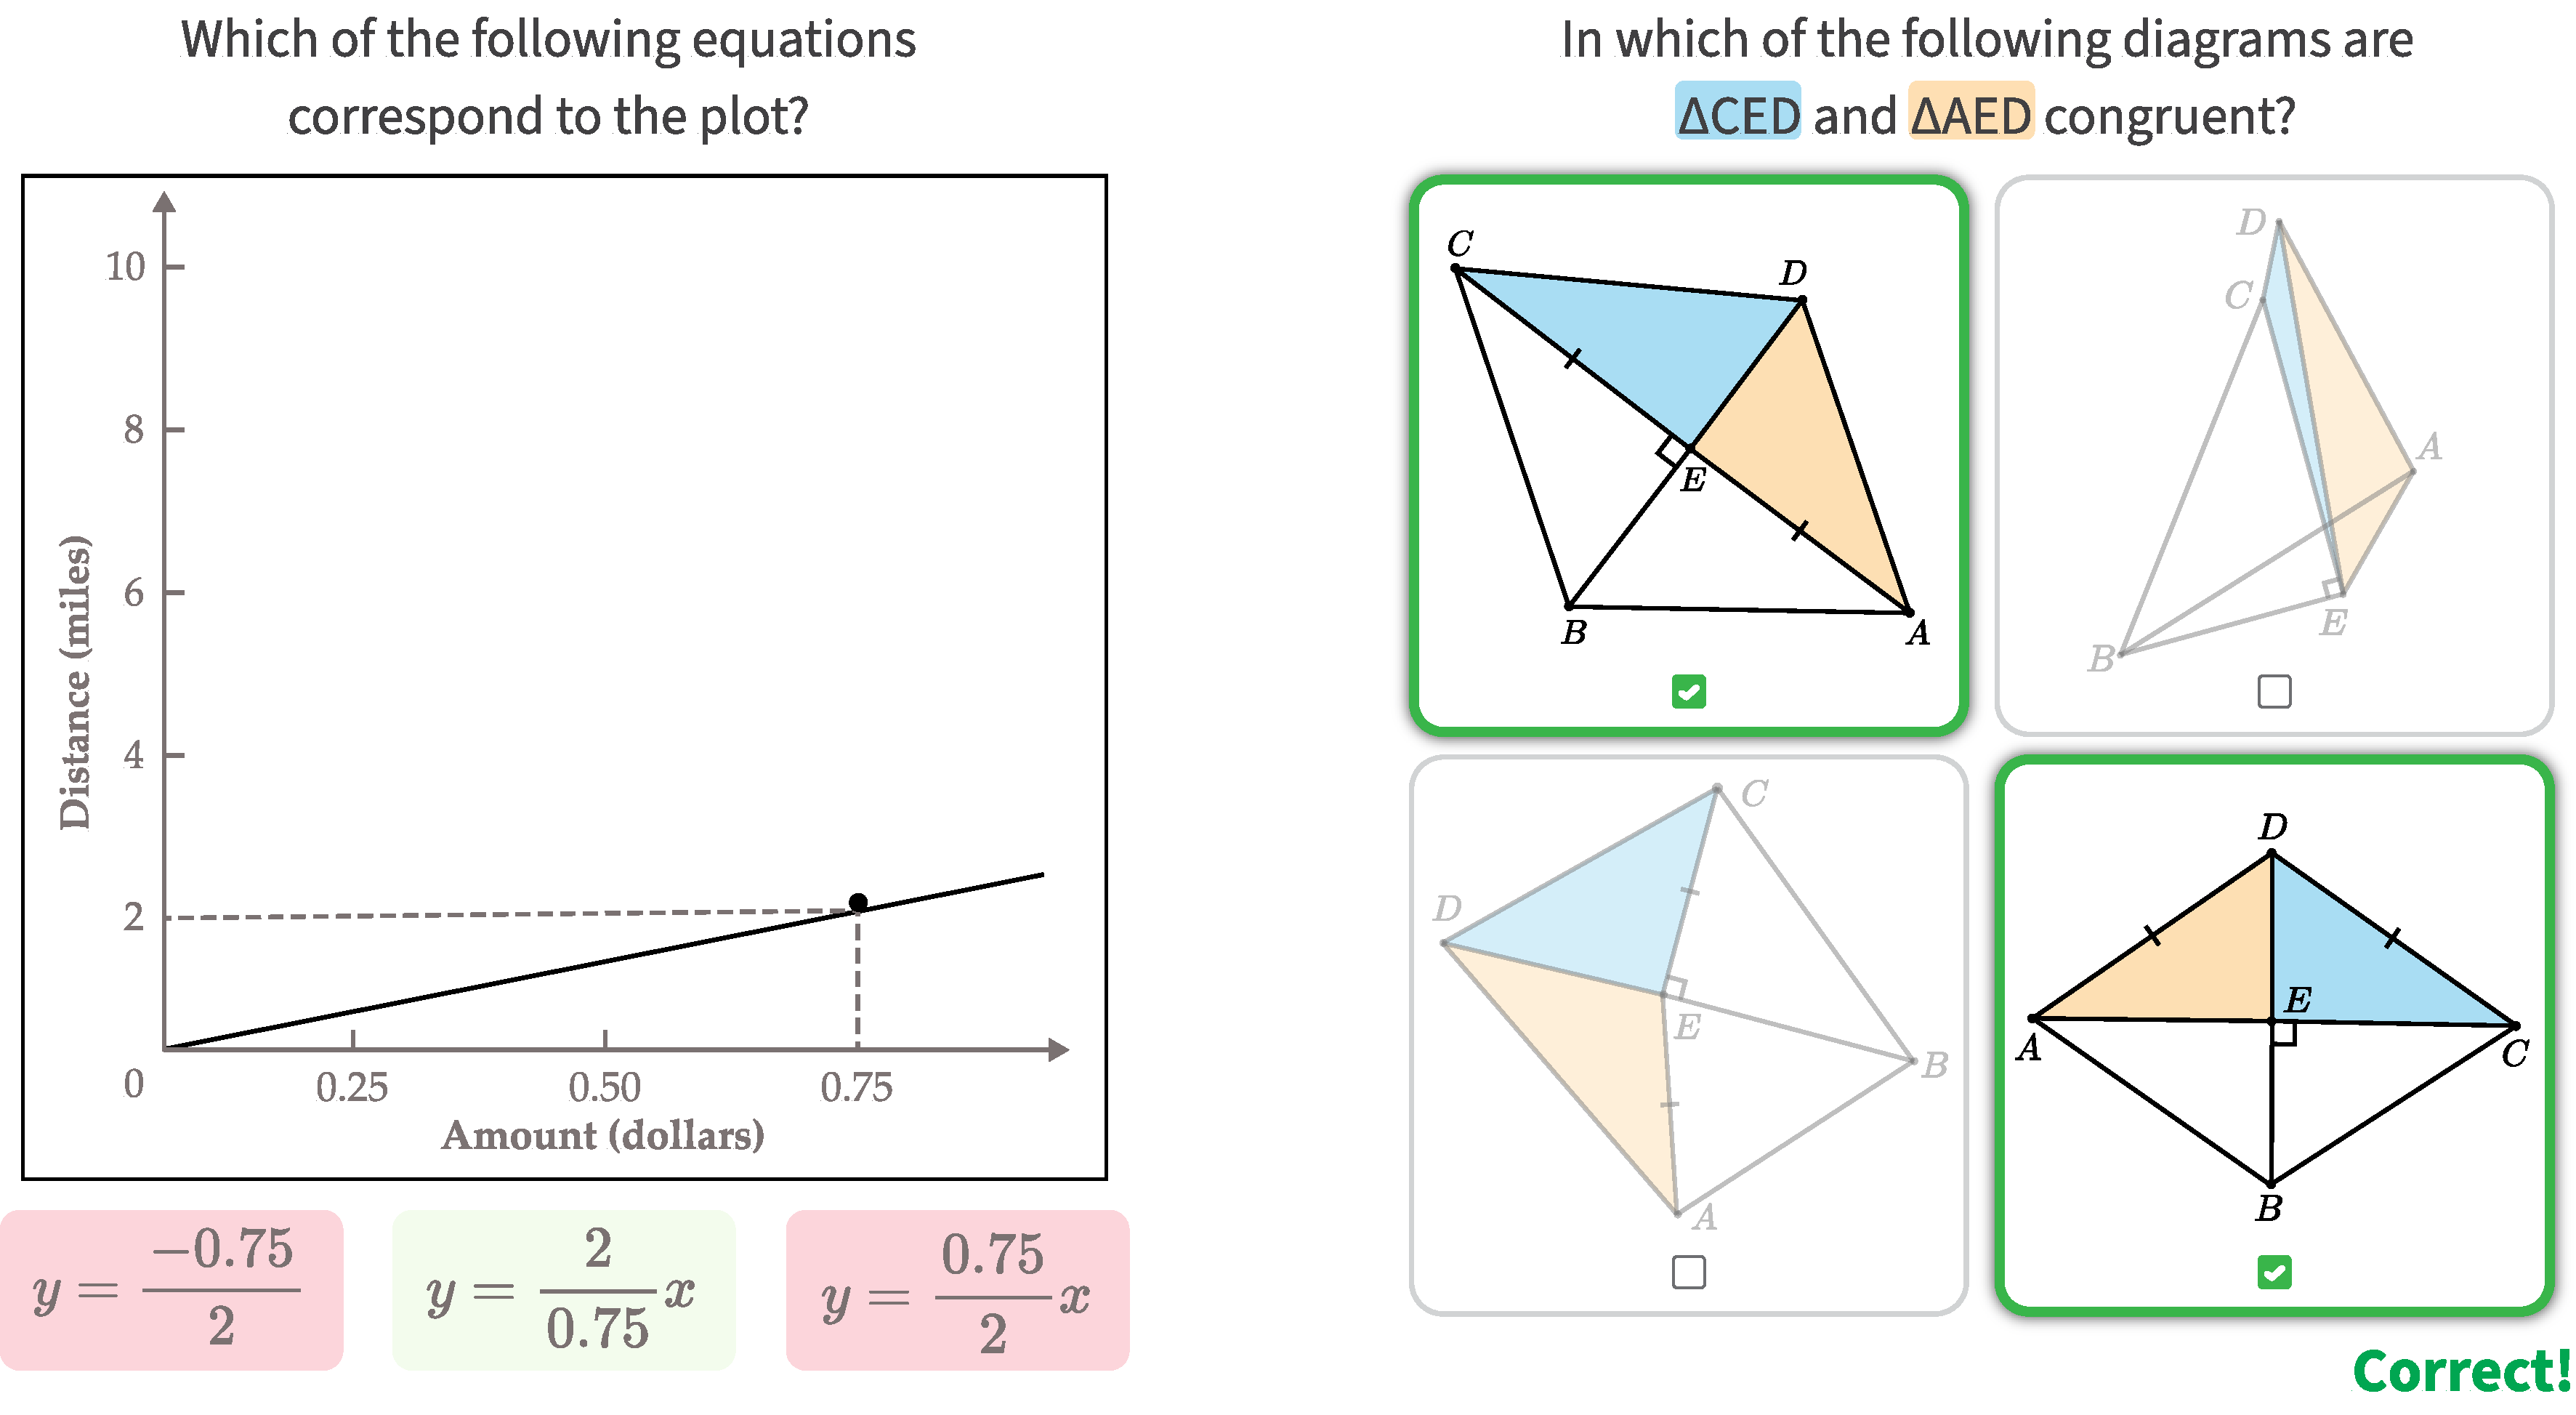
\includegraphics[width=0.88\linewidth]{assets/chapter-3/translation-problem.pdf}
    \caption{\textbf{left}: a translation problem that helps students discern the structure of linear equations (adapted from~\cite{perceptualLearning}). \textbf{right}: an \Edgeworth generated problem that trains student to recognize diagram configurations~\cite{Koedinger1990a} for triangle congruence.}
    \label{fig:translation-problem}
\end{figure}

\vspace{10pt}

\begin{figure}
    \centering
    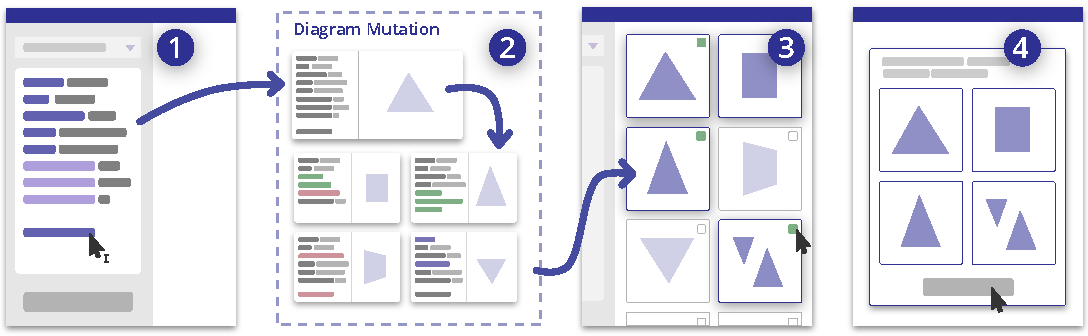
\includegraphics[width=\linewidth]{assets/chapter-3/edgeworth-teaser.pdf}
    \caption{\Edgeworth is a diagrammatic problem authoring tool that automatically generates diagram variations from a single diagram: \textmd{the author creates an example diagram~(\uilabel{1}), then \Edgeworth generates a myriad of diagram variations~(\uilabel{2}), from which the author selects diagrams~(\uilabel{3}) to form a diagrammatic multiple choice problem~(\uilabel{4}).}}
    \label{fig:teaser}
\end{figure}

Effective use of visual representations requires a certain level of \emph{representational fluency} that's achievable through deliberate practice and repetition~\cite{metarepresentation, representationalFluency}. Recognizing how words, symbols, and diagrams relate to each other is an important first step of achieving fluency. Prior work has shown that these contrasting cases, \ie, discrimination and mapping, among representations significantly improve students' ability to translate among representations~\cite{perceptualLearning}.

To train students' representational fluency, educators often create problem sets that involve numerous contrasting cases of a particular visual representation. For instance, \cref{fig:translation-problem}~shows two examples of \emph{translation problems}, where the problem asks students to determine diagrammatic \emph{instances} and \emph{noninstances} of a textual description and vice versa. Importantly, these instances and noninstances have varying degrees of differences from the given diagram or text, and carefully picking examples on this spectrum has a big impact on learning~\cite{samenessAndDifference}.

Traditionally, educators author visual practice by drawing diagrams by hand. In formative interviews (\cref{sec:edgeworth-formative}), educators reported the vital role of visual practice in their instruction, but noted the tedium of authoring due to tool limitations, leading to fewer diagrams used than desired. Manual authoring can hardly keep up with the growth of STEM learners and demand for more visual practice.

As a first step towards scaling up visual practice authoring, we built \Edgeworth, a diagrammatic problem generator. \Edgeworth generates \emph{translation problems}, an effective type of visual practice~\cite{perceptualLearning} that ask students to determine diagrammatic \emph{examples} and \emph{counterexamples} of a textual/symbolic description (\cref{fig:translation-problem}). To help authors get the most out of one diagram, \Edgeworth contributes a ``build once, generate many'' authoring paradigm: Instead of manually editing diagrams to get variations, the author creates a single diagram and \Edgeworth automatically generates diagram variations (\cref{fig:teaser}\uilabel{1}\uilabel{2}). The interaction design of \Edgeworth allows the author to visually select diagram variations to rapidly form translation problems (\cref{fig:teaser}\uilabel{3}\uilabel{4}). Given the diversity of instructional contexts in STEM, we designed \Edgeworth to be domain-agnostic: it uses a generic program mutation technique~(\cref{sec:edgeworth-mutation}) to change the author-provided diagram to produce variations. 

In this chapter, we discuss formative interviews that drove the design of \Edgeworth{} and then walk through the technical implementation of \Edgeworth.

\section{Formative interview}

\label{sec:edgeworth-formative}

We conducted semi-structured interviews with 6 educators to understand how they author, use, and maintain diagrammatic problems. We recruited participants based on their background in education and usage of diagrams in their work. Selected participants work as secondary school teachers, university professors, teaching assistants, and competitive math coaches. All participants (P1--6) indicated that they have experience creating instructional material, authoring problems, and/or developing online courses that include visual content. Example interview questions include what roles diagrams play in the participant's educational materials, how students interact with diagrams, and how diagrams are authored and maintained. The full interview protocol is included in supporting files.

Participants reported the usage of diagrams to build conceptual understanding and emphasized the need for deliberate practice to acquire representational fluency. Traditional educational materials, especially in higher education, tend to emphasize \quotei{procedures, memorization, and symbolic manipulation} (P6).  Similarly, teachers such as P1 suffer from \quotei{the curse of knowledge} of teaching visual fluency: teachers tend to \quotei{under-train} students and they struggle to use visuals for problem-solving.  As a result, students often become \quotei{symbolically good} and do not develop \quotei{good conceptual understanding} (P3). Visuals like diagrams and graphs provide alternative representations that help students \quotei{develop intuition} (P3) and \quotei{become better problem-solvers} (P4). To improve their instruction, all of our participants (P1--6) attempt to incorporate more diagrams in their instructional materials. Some also ask students to draw, annotate, and explain diagrams (P1, P2, P6). P2 encourages students to learn \quotei{multiple representations} and makes diagrams central to their math and programming curricula. When students practice with diagrams, teachers also gain richer feedback on students' level of understanding, and \quotei{learned more from this [student-drawn diagram] than 10 similar problems without the pictures} (P6).

While the benefits of and need for diagrammatic practice are clear, participants reported that tool limitations led to manual and repetitive authoring experience. Because participants typically create many problems and iterate on their content often, they face a trade-off when authoring visual content: more visuals are beneficial for learning but are time-consuming to create and modify. When authoring practice problems, P1 struggled to \quotei{create simple shapes by myself} and always ended up \quotei{copy-pasting and searching online} repeatedly. Similarly, P6 reported that they \quotei{get online images for pre-made resources, but whenever I want something a little custom, it’ll take a lot of time.} To streamline the visual authoring process, P2 and P5 developed custom pipelines for authoring problem sets and quizzes using existing programming tools. Like the problems described by prior research on diagramming tool usability~\cite{naturalDiagramming}, these tools often lack support for \quotei{high-level tweaking of my diagrams} (P2) and \quotei{are a pain to use because the language is not semantic and hard to use for non-programmers} (P5). Participants showed us many examples of tedious changes necessary to create diagram variations.

From the results, we derived the following design requirements for tool design to address participants' needs:

\begin{enumerate}[label=\textbf{D\arabic*}]
    \item\label{req:fluency} Address the need for practicing representational fluency
    \item\label{req:variation} Simplify the workflow for generating diagram variations
    \item\label{req:layout} Obviate the need to attend to low-level diagramming details
\end{enumerate}



\section{System Design of \Edgeworth}
\label{sec:system-design}


\Edgeworth realizes the design goals from \cref{sec:edgeworth-formative} by: 1) providing a domain-agnostic workflow for rapidly authoring diagrammatic practice problems (\ref{req:fluency}), 2) automatically suggesting numerous diagram variations of a single example diagram and allowing the author to visually select from the variations (\ref{req:variation}), and 3) fully automating the layout for all diagram variations (\ref{req:layout}). \cref{fig:edgeworth-interface} walks through the user interface of \Edgeworth, a simple and clean design that encapsulates the ideas above.

In \cref{sec:edgeworth-workflow}, we demonstrate the workflow of \Edgeworth by showing how to author an example diagrammatic problem in Euclidean geometry. We then describe \Edgeworth's approach to diagram layout in \cref{sec:edgeworth-layout} and how it generates diagram variation in \cref{sec:edgeworth-mutation}. 

% Finally, we discuss the limitations of the current implementation in \cref{sec:limitations}.

\begin{figure}
    \centering
    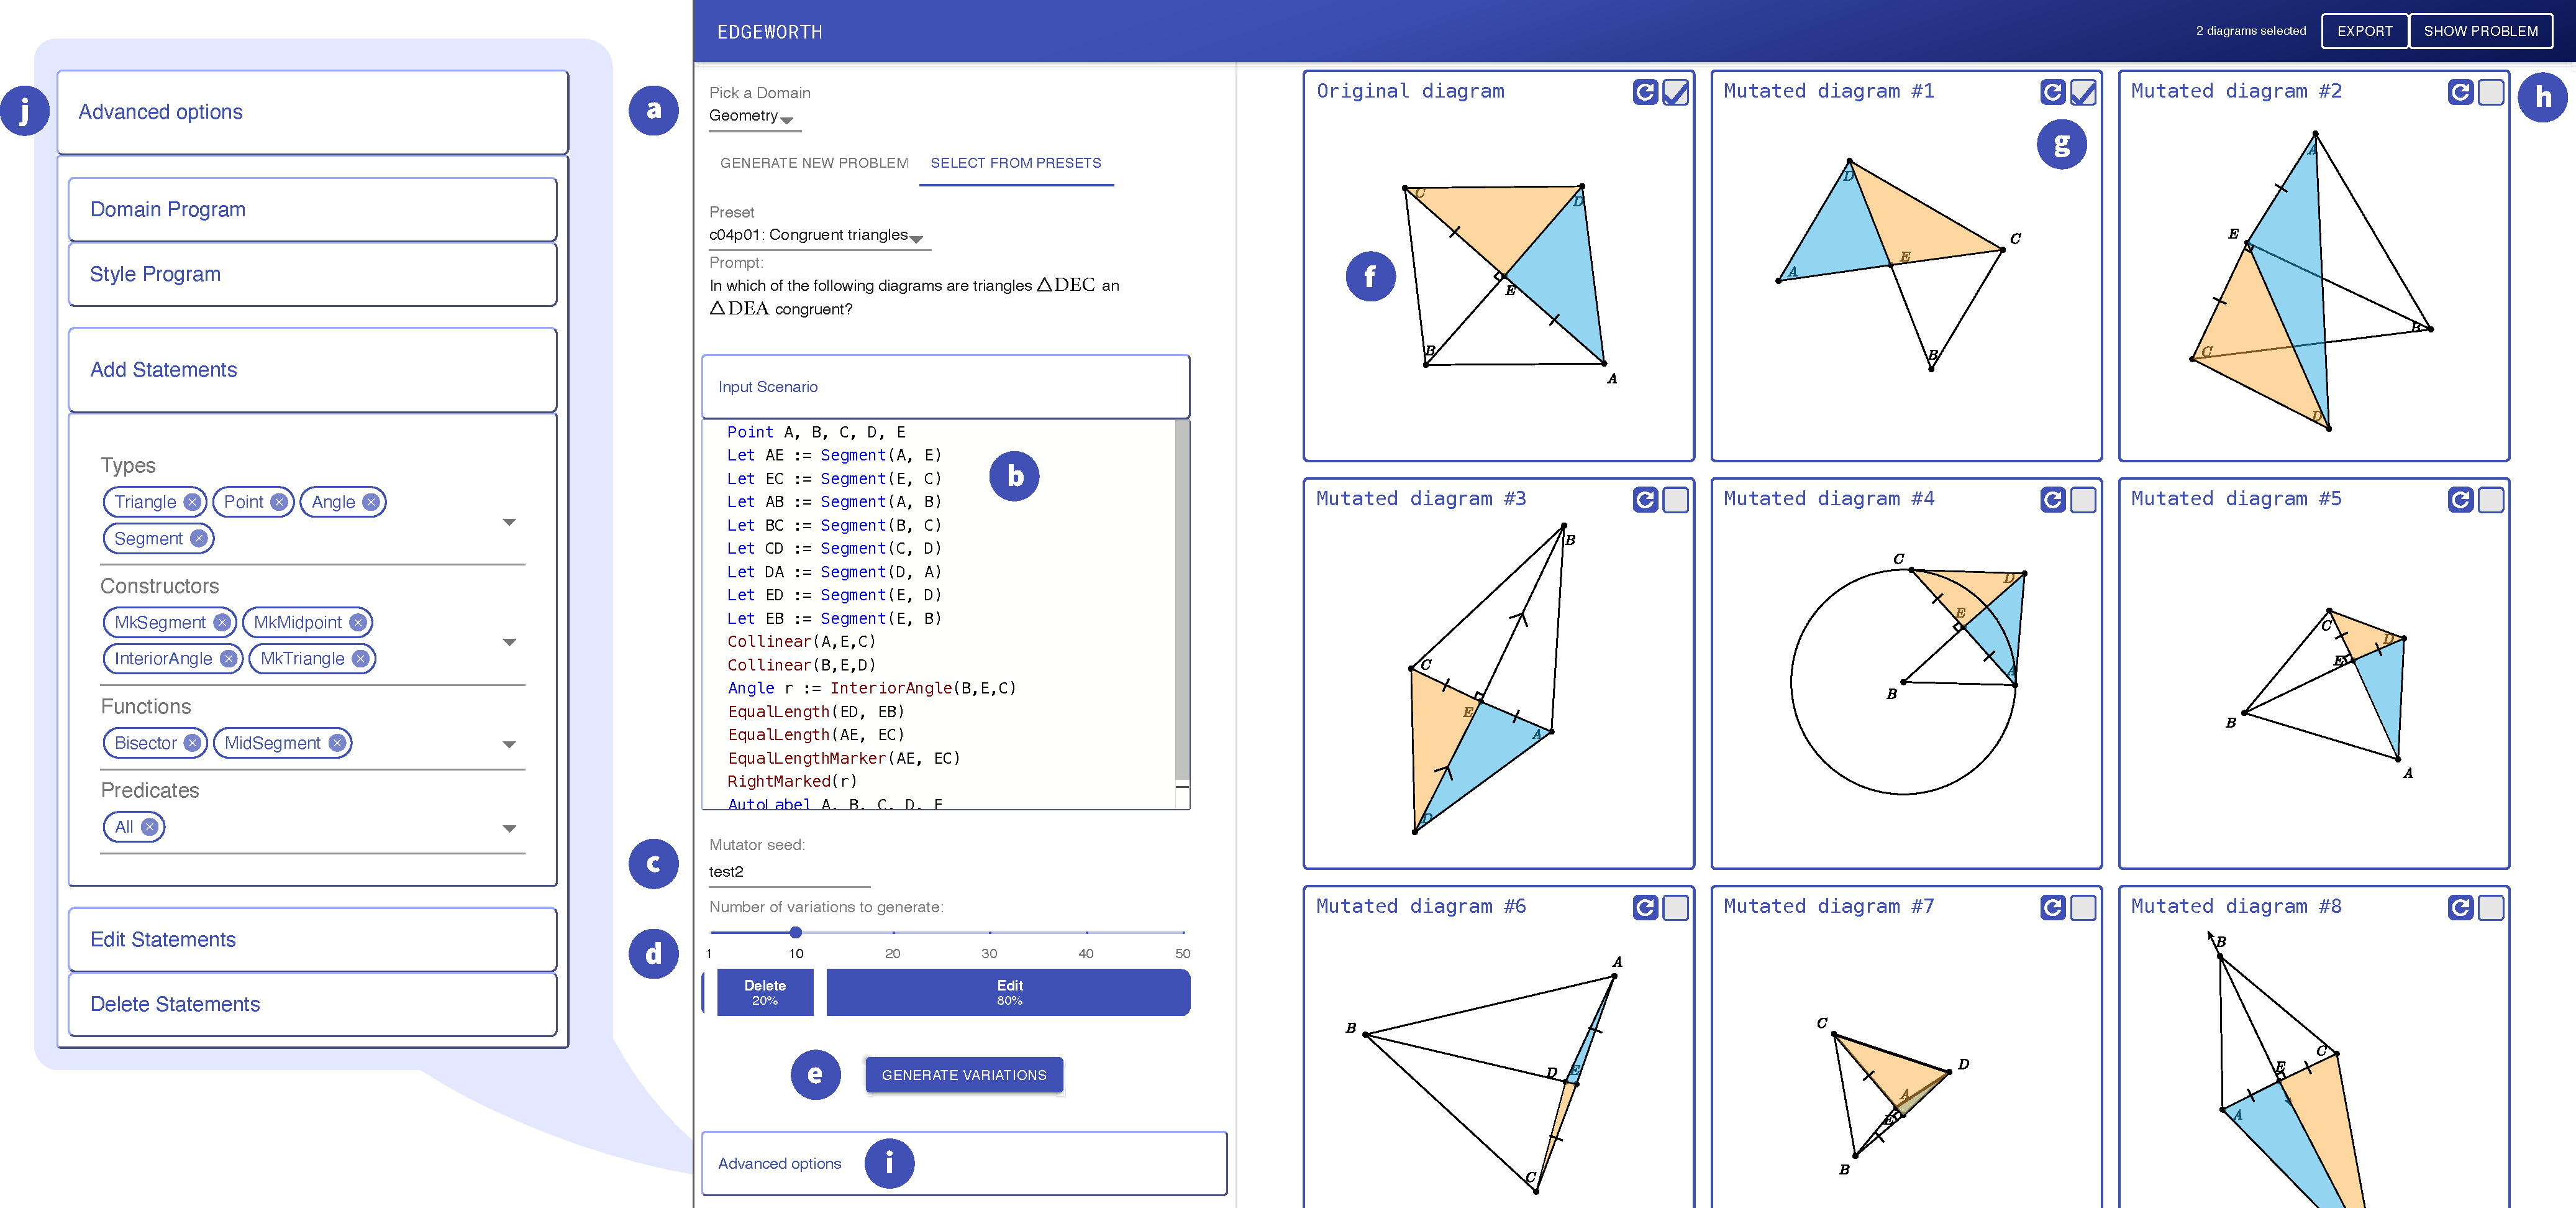
\includegraphics[width=\linewidth]{assets/chapter-3/edgeworth-ui-new.pdf}
    \caption{\textbf{The user interface of \Edgeworth.} \textmd{The author first provides a textual prompt~(\uilabel{a}) as an input scenario in \Substance notation~(\uilabel{b}). Then, clicking ``Generate Variations''~(\uilabel{e}) generates the specified number of diagram variations~(\uilabel{d}) at random based on a string seed and \hl{weights on Add, Delete or Edit mutations}~(\uilabel{c}). In the diagram panel, the top-left diagram~(\uilabel{f}) corresponds to the input scenario and the rest are diagram variations generated by \Edgeworth. The author can visually select diagrams~(\uilabel{g}) to assemble a diagrammatic multiple-choice problem~(\uilabel{h}). If needed, the author can fine-tune the mutator using ``Advanced options'' (\uilabel{i}\uilabel{j}}). }
    \label{fig:edgeworth-interface}
\end{figure}

\subsection{Author Workflow}
\label{sec:edgeworth-workflow}

In this section, we use an example from high school geometry to demonstrate the process of creating a problem in \Edgeworth. 

\subsubsection{Create an example diagram} 
\label{sec:create-scenario}

The author wants to write a problem about triangle congruence to assess students' understanding of the \textit{Side-Angle-Side} (SAS) rule. They want to create a translation problem including one diagram where the SAS rule is satisfied and three others where it is not. The author first describes an example diagram (\cref{fig:edgeworth-interface}\uilabel{b}) where this rule is satisfied. They construct a scenario involving two triangles: $\triangle DEC$ and $\triangle DEA$ share one side $DE$ and have two equal sides $EC$ and $EA$. $\angle CEB$ indicates that $AC$ and $BD$ are perpendicular and therefore $\angle DEC = \angle DEA$. Therefore, $\triangle DEC$ and $\triangle DEA$ are congruent by the SAS rule. Given this description, \Edgeworth lays out the diagram automatically (\cref{fig:edgeworth-interface}\uilabel{f}). 

% \Edgeworth mutates this scenario to create variations that may or may not satisfy the SAS rule, and the author can select from these variations to create their translation problem. While \Edgeworth requires an example scenario, it does not require it to be correct or incorrect. The choice of this scenario is specific to the format of translation problems in this problem set. Constructing the example first guarantees that there will be at least one correct choice in the problem. If the author starts with an incorrect scenario, \Edgeworth may still mutate it to create a correct choice, but it is not guaranteed.

\subsubsection{Select from \Edgeworth-generated diagrams}
\label{sec:select-diagrams}

Now the author can use \Edgeworth to mutate the example diagram by clicking ``Generate Variations'' (\cref{fig:edgeworth-interface}\uilabel{e}). \Edgeworth performs mutations on the example scenario and generates a grid of diagram variations. The grid is designed to give the author an overview of the mutation results, and diagrams are prominent in each cell to facilitate faster visual selection. The top-left cell in the grid will always display the original example diagram (\cref{fig:edgeworth-interface}\uilabel{b}\uilabel{f}), and the rest correspond to mutation results.

By inspecting each diagram in the grid, the author can determine if it is a good fit for their translation problem. If so, they click the top-right checkbox (\cref{fig:edgeworth-interface}\uilabel{g}) to include the diagram in the problem.

\subsubsection{Preview and export the problem}
After the author picks a sufficient number of diagrams (4 in this case), they can preview the translation problem by clicking ``Show Problem'' (\cref{fig:edgeworth-interface}\uilabel{h}), which displays an interactive multiple-choice widget. If the author is satisfied, they can click ``Export'' to download the diagrams and metadata to use the problem in their context. \Edgeworth exports to Scalable Vector Graphics (SVG) images for static media, source programs for interactive use, and detailed mutation trace metadata for comprehensive analysis and reference purposes.

\subsection{Diagram Notation and Layout}
\label{sec:edgeworth-layout}

\Edgeworth is built on \Penrose~\cref{chp:penrose}. Compared with alternatives, \Penrose offers two advantages: (1) a high-level diagram notation that's easy for authoring and (2) an automatic layout engine. A diagram in \Penrose consists of a textual description of the diagram content (\Substance) and a reusable layout stylesheet. 

\Substance is a simple declarative notation for describing objects and relations in a diagram. As shown in \cref{fig:cocl2-example}, \Substance has three kinds of statements: type statements (\eg \sub{Carbon c}) declare new objects; constructors (\sub{Bond b1 := MakeSingleBond(c, cl1)}) create new objects from existing objects; and predicates (\sub{ZeroValenceElectrons(c)}) indicate relations among objects. A stylesheet translates the \Substance notation to shapes and layout constraints, and then \Penrose solves for diagram layouts automatically. Since \Edgeworth authors only interact with \Substance, we omit the description of the stylesheet language in this paper; more details about stylesheets can be found in the official documentation\footnote{\url{https://penrose.cs.cmu.edu/docs}} and \citet{penrose}.

% \begin{wrapfigure}{r}{0.5\textwidth}
\begin{figure}[H]
    % \begin{center}
    \centering
    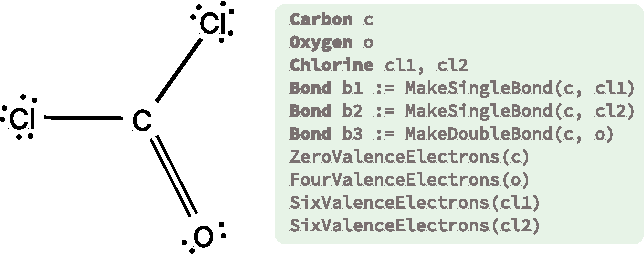
\includegraphics[width=.6\linewidth]{assets/chapter-3/cocl2-example.pdf}
    % \end{center}
    \caption{\textmd{Diagram and \Substance notation for the Lewis structure of phosgene (\ensuremath{\mathrm{COCl_2}}).}}
    \label{fig:cocl2-example}
\end{figure}

The \Penrose ecosystem offers a wide range of stylesheets for STEM diagrams, and the current \Edgeworth implementation builds on \Penrose's geometry, chemistry, and graph stylesheets for diagram layout. Since the existing \Penrose stylesheets are primarily used to generate a few human-written examples, they lack coverage for variations of \Substance descriptions required by \Edgeworth. To this end, we improved stylesheets, diagram examples, and new standard library functions to \Penrose.

\Edgeworth is the first application of \Penrose that concurrently optimizes and renders a grid of multiple diagrams. Therefore, we have made significant updates to \Penrose to support \Edgeworth's use case. To make \Edgeworth a performant client-side web application for interactive use, we have migrated from Haskell to TypeScript and made various performance improvements to efficiently run tens of layout optimization jobs in a single session. Compared to the state of \Penrose at the publication of \citet{penrose}, the development of \Edgeworth has helped improve the performance of the system by 100$\times$.


\subsection{Program Mutation}
\label{sec:edgeworth-mutation}

% what is program mutation and why it's a good fit
\Edgeworth generates diagram variations by mutating the example diagram written in \Substance. 
% what the operators are
We purposely designed the system to include a small set of simple and type-safe mutation operations. Similar to generic tree-editing algorithms~\cite{gumtree}, \Edgeworth supports 3 kinds of mutation operators: \textbf{Add}, \textbf{Delete}, and \textbf{Edit}. \textbf{Add} appends a statement. \textbf{Delete} removes a statement and all other references to that statement. 

Since compilation errors in \Substance will not produce diagrams, \textbf{Edit} involves one of the type-safe patterns listed below. Each \textbf{Edit} pattern contains a \emph{guard} and an \emph{action}. The guard checks if the operator is applicable to the given \Substance statement, and the action performs the mutation. For instance, \textbf{Replace Arguments} is only applicable when the current context has existing variables of the desired type. 
\begin{itemize}[leftmargin=*]
    \item \textbf{Swap Arguments} reorders the arguments passed into a statement; \eg if \sub{A} and \sub{B} are \sub{Triangle}s:\\
            \sub{Similar(A, B)} $\rightarrow$ \sub{Similar(B, A)}
    \item \textbf{Replace Arguments} replaces the arguments passed into a statement with other arguments defined in scope; \eg if \sub{A, B, C, D} are \sub{Point}s:\\
            \sub{s := MkSegment(A, B)} 	$\rightarrow$ \sub{s := MkSegment(C, D)}
    \item \textbf{Replace Function} replaces a statement with a different statement that takes the same arguments; \eg if \sub{T} is a \sub{Triangle} and \sub{E} is an \sub{Angle}:\\
            \sub{Equilateral(T)} $\rightarrow$ \sub{Scalene(T)} \\
            \sub{Segment s := Bisector(E)} $\rightarrow$ \sub{RightAngleMarked(E)}
\end{itemize}

% one-col
\begin{algorithm}
\caption{The \Edgeworth mutation algorithm. }\label{alg:mutation}
\begin{algorithmic}[1]
\Function{Generate}{$p, \ell, h, a, d, e, A, D, E$}
\State $p' \gets p$
\State $n \gets \text{uniform random integer between $\ell$ and $h$}$\label{line:mutations}
\For{$i$ \textbf{from} $1$ \textbf{to} $n$}
    \State $x \gets \text{uniform random real between $0$ and $a + d + e$}$\label{line:kind}
    \If{$x < a$}
        \State $m \gets \textsc{RandomAdd}(A, p')$\label{line:add}
    \ElsIf{$x < a + d$}
        \State $m \gets \textsc{RandomDelete}(D, p')$\label{line:delete}
    \Else
        \State{$s \gets \text{uniform random element of $\textsc{Statements}(p')$}$}\label{line:statements}
        \State{$m \gets \textsc{RandomEdit}(E, s)$}\label{line:edit}
    \EndIf
    \State $p' \gets \textsc{Mutate}(p', m)$
\EndFor
\State \textbf{return} $p'$
\EndFunction
\end{algorithmic}
\end{algorithm}
% one-col

Algorithm~\ref{alg:mutation} shows how the \Edgeworth mutator works, at a high level. In addition to the input \Substance description $p$, \Edgeworth also takes a number of user-defined configuration parameters: (1) a number of variations to generate (the number of times \textsc{Generate} is called); (2) a range of mutation counts per variation (the input variables $\ell$ and $h$); (3) weights for \textbf{Add}, \textbf{Delete}, and \textbf{Edit} operations (the input variables $a$, $d$, and $e$ respectively); and (4) filter sets $A$, $D$, and $E$ which limit the set of mutations that the \textbf{Add}, \textbf{Delete}, and \textbf{Edit} operations can produce.

% how the mutator produces mutants
Given an example diagram, \Edgeworth performs several rounds of mutation generation. Each round results in a series of mutations that alter the input to produce a variation. The number of mutations (line~\ref{line:mutations}) is bounded by the configuration parameters.

To generate a single mutation, \Edgeworth makes a weighted choice (line~\ref{line:kind}) of the mutation kinds and enumerates all possible mutations for the chosen kind: \textbf{Add} enumerates all possible statements to add (line~\ref{line:add}); \textbf{Delete} randomly deletes an existing statement (line~\ref{line:delete}); \textbf{Edit} enumerates all possible edits for all statements (line~\ref{line:statements}) and picks one of them randomly (line~\ref{line:edit}). The randomness of \Edgeworth is controlled by a single random generator seed.

Users can specify filter sets under the ``Advanced options'' section of the UI, shown in \cref{fig:edgeworth-interface}\uilabel{i}\uilabel{j}. The filters default to ``All,'' which indicates that the mutator may change any statement in the example diagram. While this precise configuration may be useful, we ended up not using them in our evaluation (\cref{chp:edgeworth-eval}) and instead achieving our results using only \Edgeworth's simpler core set of configuration options, i.e., weights on mutation operators.

% \section{Mutation-based diagram generation}
% \label{sec:edgeworth-mutation}

% Educators simply don't have enough time to produce good-looking diagrams, not to mention the amount and variety of diagrams required for training students to be fluent in visual representations. Therefore, a key pain point to automate is diagram generation. Importantly, the generated diagrams have to be meaningful and need to include contrasting cases of the same subject matter. 

% In \Edgeworth, I propose to \textbf{generate a large pool of diagrams by mutating the \Substance program in a \Penrose trio}. Compared with general-purpose programming languages, \Penrose DSLs have unique advantages: \Domain is a meta-language that precisely defines the available program constructs in \Substance, which helps define the mutation search space. Moreover, it’s easier to make sense of mutation on \Substance, because it corresponds to the domain-specific vocabulary of diagram authors. 

% At a high level, the \Edgeworth mutator takes in a \Penrose trio and a small configuration file, and simply generates an arbitrary number of \Substance programs. Constrained by the configuration, \Edgeworth mutates the \Substance program (\emph{prompt program}) by applying a series of program mutations to get a \emph{mutant} \Substance program. For each mutant, the system then uses the original \Style and \Domain programs to render a diagram. 
 
% \begin{figure}[h]
%     \centering
%     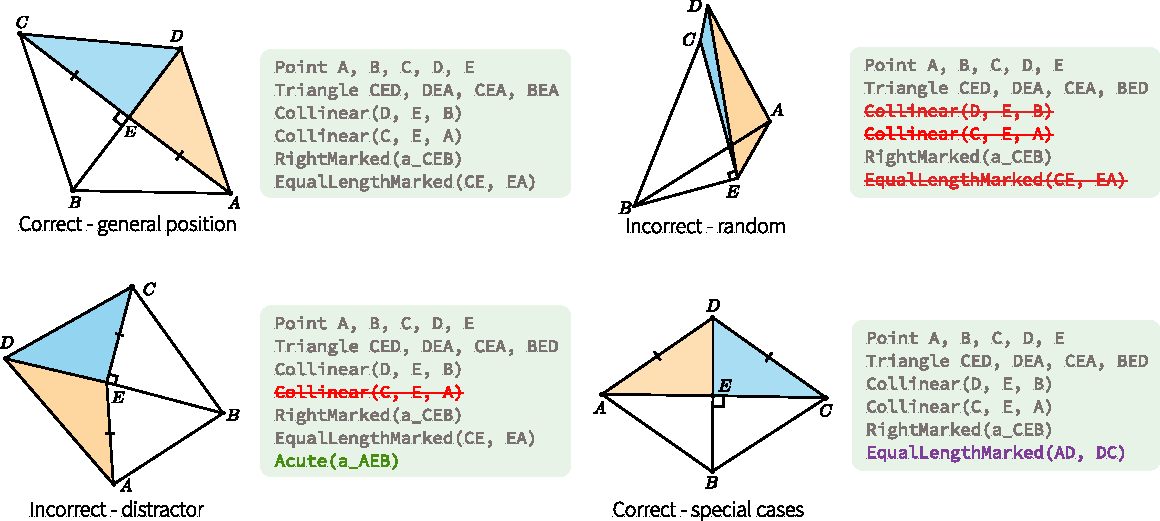
\includegraphics[width=\linewidth]{assets/chapter-3/answer-types.pdf}
%     \caption{Four example classes of mutants generated by \Edgeworth. \textbf{Top-left}: the original prompt program, representing a general correct instance. \textbf{Bottom-Left}: an incorrect noninstance that only slightly differs from the original prompt semantically. \textbf{Top-right}: an incorrect noninstance that differs significantly from the prompt. \textbf{Bottom-right}: a correct instance that's a corner-case of the prompt.}
%     \label{fig:answer-types}
% \end{figure}

% Since \Substance is a small declarative language, \Edgeworth uses a set of pre-defined, high-level mutation operations listed below. 

% \begin{itemize}
%     \item \textbf{Add} Appends a statement to the \Substance program.
%     \item \textbf{Delete} Removes a random statement from the \Substance program.
%     \item \textbf{Cascading Delete} Removes a random statement and all other references to that statement.
%     \item \textbf{Swap Arguments} Reorders the arguments passed into a statement. \eg, if \sub{A} and \sub{B} are \sub{Triangles}:
    
%             \sub{Similar(A, B)} $\rightarrow$ \sub{Similar(B, A)}
%     \item \textbf{Swap-In Arguments} Replaces the arguments passed into a statement with other arguments defined in scope. \eg, if \sub{A, B, C, D} are \sub{Points}:
            
%             \sub{s := MkSegment(A, B)} 	$\rightarrow$ \sub{s := MkSegment(C, D)}
%     \item \textbf{Replace Statement Name} Replaces a statement with a different statement that takes the same type of arguments and has the same return type. \eg, given that \sub{T} is a \sub{Triangle}:
            
%             \sub{Right(T)} $\rightarrow$ \sub{Obtuse(T)}
%     \item \textbf{Type Change} Replaces a statement with a new one that takes the same number and type of arguments, but does not necessarily return a value of the same type. \eg, if \sub{E} is an \sub{Angle}:
            
%             \sub{Segment s := Bisector(E)} $\rightarrow$ \sub{Right(E)}
% \end{itemize}

% These mutations are all done safely at the level of the abstract syntax tree (AST) and \Edgeworth maintains a local context and symbol table, so operations will not introduce errors. The configuration file contains a set of rules to filter down the search space by statement types and specify the kinds of mutations allowed. 

% Authoring contrasting cases require different classes of diagrams: those that correctly correspond to the textual/symbolic description and others that don't. Importantly, nearest neighbors of the prompt program seem to have great education values, \ie, ``near misses'' and ``near hits.'' Knowing the correctness of a mutant also helps with automated grading of problems. 

% Although \Edgeworth generates syntactically valid mutants, the system doesn't know whether a mutant is semantically consistent with the prompt \apriori. Currently, the system uses the graphical constraints to determine semantic consistency. Specifically, it uses an energy-based heuristic by performing \textbf{cross-instance energy evaluation (CIEE)} of each mutant. Suppose \Edgeworth mutates the prompt program $P$ to mutant $P'$ and generates a diagram $D'$ from $P'$. the system can compute the cross-instance energy of $D'$ by 1) checking if all of the constraints generated from $P$ are met by $D'$ and 2) run the objective function defined by $P$ on $D'$ and check if the $D'$ is at a local minimum.  In other words, the \Penrose optimizer determines if the diagram $D'$ generated from mutated program $P'$ is a good fit for the prompt program.

% \vspace{10pt}

% \begin{figure}[h]
%     \centering
%     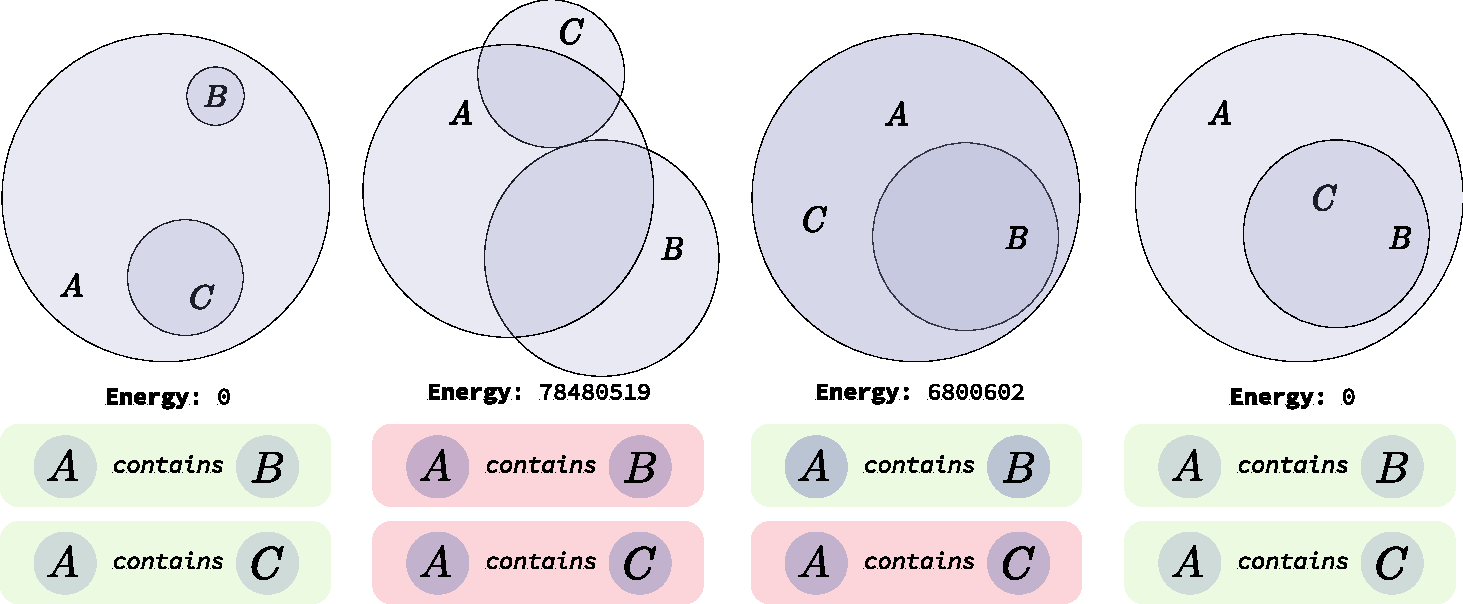
\includegraphics[width=\linewidth]{assets/chapter-3/ciee.pdf}
%     \caption{An example of CIEE, where the leftmost is the prompt program $P$ and its corresponding diagram $D$. The overall energy value is $0$. The right three are instances of $P'$, on which the constraints from the prompt are evaluated. The middle two are \textit{semantically inconsistent} with the prompt and have high energy values. The rightmost is \textit{semantically consistent} with the prompt and therefore has an energy value of $0$.}
%     \label{fig:ciee}
% \end{figure}

% \vspace{10pt}

% \begin{proposed}
% \textbf{CIEE robustness.} CIEE showed some promise on a limited set of examples, but further evaluation is needed to see the robustness of this heuristic. For instance, how much does this method depend on the qualities of the \Style program that defined the constraints? If the mutant significantly differs from the prompt (\eg, missing most identifiers from the prompt), is this heuristic still useful?

% \textbf{\Domain language extensions.} None of the predefined mutations listed above carry any mathematical semantics because \Domain doesn't contain enough information. For instance, many mathematical predicates have reflexive, symmetric, transitive, and substitution properties, but \Domain only encodes basic type definitions. For a more precise notion of correctness, I plan to extend \Domain to model such properties, and use them in the \Edgeworth mutator, possibly together with CIEE, to generate higher quality mutants.  

% \end{proposed}

% \section{Preliminary evaluation of the \Edgeworth mutator}
% \label{sec:edgeworth-prelim-eval}

% In preliminary work, we evaluated the system by recreating problems in a middle-school geometry textbook \cite{holtGeometry}. We examined all 53 diagrammatic problems in the chapter review sections and picked a representative subset of 24 problems and implemented them in \Edgeworth. For each textbook problem, the prompt is reframed so that the diagram accompanying the original problem can be considered a correct answer. Then, we consider possible answers to the posed question, including ``distractors''---answers that are designed to tempt students with limited conceptual understanding---as well as correct ``special cases''. We then describe the original diagram as a prompt \Substance program and pass it to \Edgeworth, which generates numerous answers to the original problem.

% We examined sets of 20 diagrams generated by \Edgeworth based on various prompt programs. Each program was mutated 1-3 times and the correctness of each diagram was determined manually. We found that while \Edgeworth easily generates a variety of correct and incorrect diagrams, careful selection of configuration parameters was often required to get more ``interesting'' diagrams (correct special cases, distractors).

% \begin{proposed}
% \label{prop:config-usability}
% \textbf{Usability of the \Edgeworth configuration.} As noted above, results from the \Edgeworth mutator are sensitive to the configuration. For instance, a statement in the \Substance program might be particularly more suitable for mutations than others (perhaps because it contributes to the correctness of the problem.) Under- or over-specifying mutations in the configuration might lead to a pool of ``noisy'' diagrams. I propose to conduct a light-weight case study with a handful of problems to identify the key to successful configurations. With that insight, we can either improve the configuration format or explore other modes of interaction.
% \end{proposed}

% \section{Mutation paths as problem templates}
% \label{sec:edgeworth-mutation-paths}

% \begin{proposed}
% After generating a pool of diagrams, the author then picks a subset of them for a single \emph{problem instance}. For each generated diagram, \Edgeworth keeps a record of the series of mutations performed on the prompt program (\emph{mutation path}) to the mutant. For a multiple choice problem with four options, there will be four mutation paths from the prompt. Together these paths form a \emph{problem template}.

% A problem template is specific to a prompt, so it's unlikely to be reusable for generating other problem instances. However, many problems might share the same instructional goal such as teaching students the conditions for the Hypotenuse-Leg (HL) theorem. While the choice of names and diagram design may differ, the core structure is the same: two instances of congruent triangles satisfying HL and two noninstances of non-congruent triangles. Encoding this information can further scale up problem authoring. 

% I propose to \textbf{investigate common structures among problem templates and encode them as problem template specifications that are generalizable to multiple prompts}. 

% \end{proposed}

% \section{By-example workflow for authoring at scale}
% \label{sec:edgeworth-by-example}

% With the \Edgeworth mutator, the primary mode of interaction is picking examples from the mutant pool and editing the configuration to narrow down the search space. In some cases (see \cref{prop:config-usability}), the author might want to write a few examples from scratch, or prefer to manually make slight tweaks to examples in the mutant pool. I propose to \textbf{create a programming-by-example workflow, where the author manually creates a few diagrams and \Edgeworth generates a bigger pool of diagrams with similar properties}.

% \vspace{10pt}
% \begin{figure}[h]
%     \centering
%     \includegraphics[width=\linewidth]{assets/chapter-3/synthesis-driven-workflow.pdf}
%     \caption{User interface mock-up of a by-example workflow in \Edgeworth.}
%     \label{fig:synthesis-driven-workflow}
% \end{figure}
% \vspace{10pt}

% For example, if \Edgeworth fails to generate a pool of useful diagrams, the author can manually create a few examples by directly editing the prompt program. In \cref{fig:synthesis-driven-workflow}, the author adds the \sub{Equal(B, C)} predicate. Their intent is to include the edge case of proper subsets in this problem, where some of the subset relations are actually equality. \Edgeworth generates a set of similar examples that add \sub{Equal} predicates with existing identifiers in different ways. 

% The addition of \sub{Equal(B, C)} is effectively a user-generated mutation, and \Edgeworth needs to understand this mutation to generate similar instances. Currently, the \Edgeworth synthesizer matches a series of author edits to predefined mutations. Once the synthesizer finds a path, it can then inform the mutator to generate examples with similar properties (\ie, including the edge case of equal sets). 

% \begin{proposed}
% \textbf{Generalized mutation paths} Similar to templates, the by-example workflow also requires a generalizable encoding of mutations. I plan to experiment with a few possible formats such as (1) another mutator configuration and (2) mutation paths with ``holes.''
% \end{proposed}

% \section{Evaluation}

% \begin{proposed}
% \textbf{Usability study of \Edgeworth.} I propose to evaluate the usability of \Edgeworth by recruiting authors to perform content authoring tasks with the \Edgeworth prototype. For example, the participants may be asked to author a problem set of 10 diagrammatic problems. The goal of this study will be to identify missing features, usability problems, and opportunities for simplification. The study may include several rounds with increasingly high-fidelity prototypes. After each round, I will refine the design and implement the next prototype. Here are some possible research questions:
% \begin{itemize}
%     \item  What are the key design considerations for diagrammatic problem authoring? How do they fit with the features of \Edgeworth?
%     \item How do authors prefer to work with \Edgeworth? When do they opt to write a configuration file and generate many diagrams? When do they use the by-example workflow? Do they mix the two workflows?
%     \item How does the experience compare to their existing tools? How can \Edgeworth incorporate useful parts of them? 
% \end{itemize}
% \end{proposed}


\chapter{\Edgeworth{} Usability Evaluation}

\section{Definitions}
\label{sec:definitions}

In the discussion of translation problems, \cref{chp:edgeworth} uses terms such as ``instance,'' ``noninstance,'' ``near hit,'' and ``near miss.'' To standardize the terminologies in this appendix, I give some definitions here.

Given a set of mathematical statements describing logical entities and their relationships, a diagram can be associated with them in one of the following ways:

\vspace{0.5em}
\begin{figure}[h]
\begin{minipage}[b]{0.48\linewidth}
$\bullet$ \textbf{Example}: the diagram represents the math statements, \ie all the statements hold true in the diagram. 
    \vspace{3pt}
    
$\bullet$ \textbf{Counterexample}: the diagram clearly violates the math statements, \ie one or more statements are false in the diagram.
    \vspace{3pt}
    
$\bullet$ \textbf{Positive edge case}: the diagram is an example of the math statements, but contains extraneous entities and/or more specialized relationships. 
    \vspace{3pt}
    
$\bullet$ \textbf{Negative edge case}: the diagram is a counterexample, but only requires a few changes to become an example.
\end{minipage}
\hfill
\begin{minipage}[b]{0.45\linewidth}
    \centering
    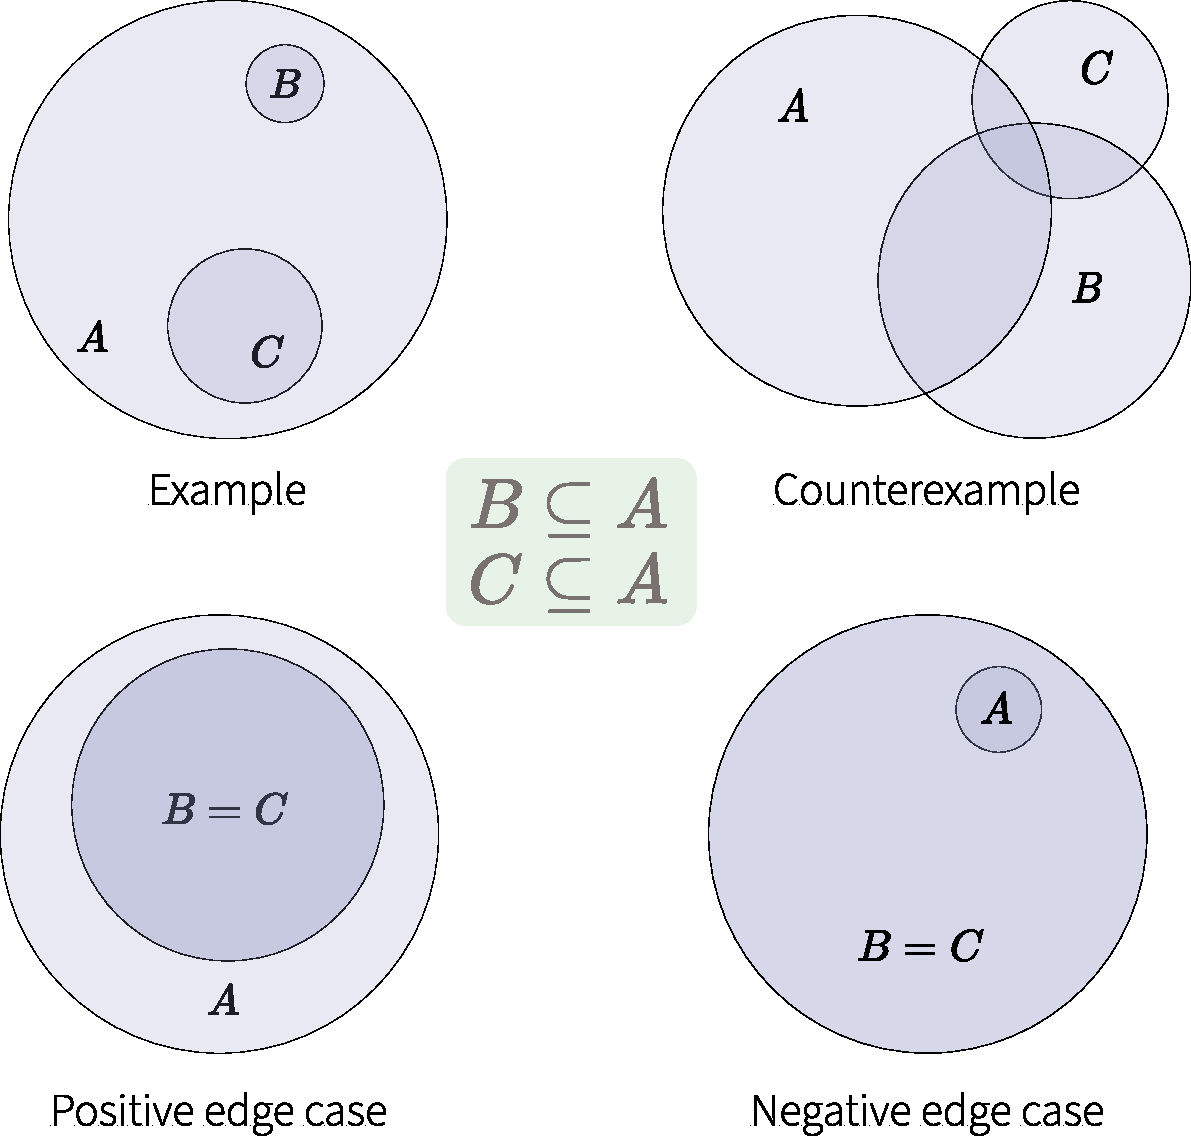
\includegraphics[width=\textwidth]{assets/appendix/definitions-examples.pdf}
\end{minipage}
\end{figure}

% While distinguishing between examples and counterexamples is often straightforward, identifying edge cases can depend on the context. For instance, the counterexamples in the figure above both violate all math statements, but the lower-right diagram can be considered an edge case because one can swap the labels $A$ and $B$ to make it an example. 

\section{Summary of proposed work}

\subsection{Programming-by-example workflow}


\begin{figure}
    \centering
    \includegraphics[width=\linewidth]{assets/appendix/edgeworth-bad-output.pdf}
    \caption{A screenshot of the \Edgeworth interface, after generating examples for a translation problem focusing on improper subsets. Because of the configuration, pool of mutant diagrams aren't suitable for this problem.}
    \label{fig:edgeworth-bad-output}
\end{figure}


With the \Edgeworth mutator, the primary mode of interaction is configuration-based: the author creates a mutator configuration and the mutator generates a set of diagrams. When these diagrams don't satisfy the needs of the author (\eg missing counterexamples that are important for an educational goal), the author can only edit the configuration again and hope to get better ones. In short, the quality of \Edgeworth-generated diagrams are sensitive to the configuration. 

For example, suppose an author would like to create translation problems that test students' knowledge of improper subsets, especially the fact that if $A \subseteq B$, $A = B$ is allowed. Using the \Edgeworth mutator, the author first creates a prompt \Substance program:

\begin{verbatim}
Set A, B, C
IsSubSet(B, A)
IsSubset(C, A)
\end{verbatim}

Not familiar with how program mutator works, the author picks a few options in the configuration interface and clicks ``Generate Diagrams.'' Ideally, \Edgeworth should generate a set of examples of the subset relations that include the edge cases of $A = B$, $A = C$, or $B = C$, and counterexamples of $B \not\subseteq A$ or $C \not\subseteq A$. 

However, the output from \Edgeworth seems too random (\cref{fig:edgeworth-bad-output}). There are useful counterexamples, but none of the diagrams include edge cases such as:
\begin{verbatim}
Set A, B, C
IsSubSet(B, A)
IsSubset(C, A)
Equal(B, C)
\end{verbatim}

In other words, without intimate knowledge of how the \Edgeworth mutator is configured, the author cannot express their intent easily. In this case, it's much more natural to write a few examples from scratch, or manually make slight tweaks to examples in the mutant pool. I propose to \textbf{create a programming-by-example (PBE) workflow, where the author manually creates or edits a few diagrams, and \Edgeworth generates more diagrams with similar properties.}

Using this workflow for the example above, the author can manually create a few examples by directly editing the prompt program. In this case, the author adds the \sub{Equal(B, C)} predicate. Their intent is to include the edge case of improper subsets in this problem, where some of the subset relations are actually equality. \Edgeworth generates a set of similar examples that add \sub{Equal} predicates with existing identifiers in different ways. 

\vspace{10pt}
\begin{figure}[h]
    \centering
    \includegraphics[width=0.8\linewidth]{assets/appendix/synthesis-driven-workflow.pdf}
    % \caption{Caption}
    % \label{fig:my_label}
\end{figure}
\vspace{10pt}

The addition of \sub{Equal(B, C)} is effectively a user-generated mutation, and \Edgeworth needs to understand this mutation to generate similar instances. To do so, the \Edgeworth synthesizer matches a series of author edits to predefined mutations. Once the synthesizer finds a mutation path that describes the author edit, it can then inform the mutator to generate examples with similar properties (\ie including the edge case of equal sets). Using this workflow, the author can rapidly author diagrams that belong to a particular category in the translation problem. For example, the problem below has diagrams that include set equalities as correct answers, and diagrams that violate one or both subset relations as incorrect answers.

\vspace{10pt}
\begin{figure}[h]
    \centering
    \includegraphics[width=0.8\linewidth]{assets/appendix/translation-problem-sets.pdf}
    % \caption{Caption}
    % \label{fig:my_label}
\end{figure}
\vspace{10pt}

\subsection{Automatic detection of examples and counterexamples}
\label{sec:autodetect}

One key application of \Edgeworth is generating translation problems with examples and counterexamples. Therefore, it's important for the system to understand whether a diagram is an example or counterexample of the prompt. However, the \Edgeworth mutator performs \Substance program mutations on the prompt without knowing if a mutant is semantically equivalent to the prompt. To address this, I propose to \textbf{automatically detect examples and counterexamples}.

One heuristic is cross-instance energy evaluation (CIEE) described in~\cref{sec:mutation}.  CIEE determines the distance between two \Substance programs by examining visual constraint satisfaction. 

Another approach is to provide the \Edgeworth mutator with more semantic information such that it generates examples and counterexamples by construction. Currently, none of the mutation operators carry any mathematical semantics because \Domain doesn't contain enough information. For instance, many mathematical predicates have reflexive, symmetric, transitive, and substitution properties, but \Domain only encodes basic type definitions. For a more precise notion of correctness, I plan to extend \Domain to model such properties, and use them in the \Edgeworth mutator, possibly together with CIEE, to generate higher quality mutants.  

\subsection{Hypotheses and research questions}

Comparing with related work discussed in \cref{sec:edgeworth-related}, \Edgeworth uniquely support scalable generation of diagrammatic translation problems in multiple domains. Therefore, in this section, I discuss hypotheses that cover the essential features of \Edgeworth such as the mutation-based approach and automatic detection of examples and counterexamples. For each hypothesis, I will also discuss further research questions to be investigated in the evaluation plan. 

\boxtext{\textbf{H1:} Given manageable effort in configuring the mutator, \Edgeworth can reliably generate examples and counterexamples for translation problems with relatively few mutants required.}

An effective translation problem needs to include both examples and counterexamples. Therefore, the technical approach of \Edgeworth---program mutations on \Substance code---must produce them reliably. To verify H1, the following research questions need to be answered:

\begin{itemize}
    \item \textbf{R1.1}: How many mutants does \Edgeworth need to generate to obtain sufficient examples and counterexamples for translation problems?
    \item \textbf{R1.2}: How frequently does \Edgeworth succeed or fail at doing so?
\end{itemize}

The preliminary evaluation showed that the mutator configuration will affect the quality of the mutants. Therefore, I will also address the following research question on mutator configuration and will use the results to further investigate possible ways to lower the configuration burden, e.g. the programming-by-example workflow and changes to the configuration format.

\begin{itemize}
    \item \textbf{R1.3}: How much configuration effort is required to produce examples and counterexamples? 
\end{itemize}

\boxtext{\textbf{H2}: \Edgeworth makes translation problem authoring more efficient.}

The main goal of \Edgeworth is to improve the efficiency of translation problem authoring. To verify H2, the evaluation plan will answer:
\begin{itemize}
    \item  \textbf{R2.1}: Comparing with workflows that authors are using, can \Edgeworth shorten the authoring time of translation problems?
    \item  \textbf{R2.2}: Which aspect(s) of the authoring workflow does \Edgeworth simplify, and does \Edgeworth introduce new authoring difficulties? 
    \item  \textbf{R2.3}: Are authors more efficient using the configuration-based workflow or programming-by-example workflow?
\end{itemize}

Regardless of the answer to R2.1, meaningful results on R2.2 can provide more insights on how \Edgeworth's approach impacts the problem authoring experience. For instance, I postulate that \Edgeworth improves authoring efficiency by (1) simplifying the mechanics of diagram production and (2) reducing the author's effort to come up with examples and counterexamples. On the other hand, \Edgeworth's mutation-based approach may introduce new problems such as difficulties finding the right diagrams from the mutant pool and controlling the quality of examples. The automatic detection heuristics described above aim to mitigate these difficulties.

\boxtext{\textbf{H3}: \Edgeworth can automatically distinguish examples from counterexamples, and this feature helps authors find examples and counterexamples for translation problems.}

The effectiveness of translation problems depends on the choice of examples and counterexamples. I hypothesize that example generation/selection is a nontrivial activity that authors spend time doing, and computational support in \Edgeworth can help authors identify examples/counterexamples. Answering the following research questions will verify H3:

\begin{itemize}
    \item \textbf{R3.1}: Can \Edgeworth automatically detect examples, counterexamples, and edge cases with a reasonably high accuracy?
    \item \textbf{R3.2}: Do the detection results help authors identify potential answers to translation problems?
\end{itemize}


\section{Plan}

\subsection{Pilot usability evaluation}

To prepare the \Edgeworth prototype for evaluation, I will first evaluate the usability of \Edgeworth by recruiting authors to perform small authoring tasks with the \Edgeworth prototype. For example, the participants may be asked to author a simple diagrammatic translation problem. The goal of this pilot study is to identify missing features, usability problems, and opportunities for simplification. The study may include several rounds with increasingly high-fidelity prototypes. After each round, I will refine the design and implement the next prototype. Here are some possible high-level questions for the study:
\begin{itemize}
    \item What are the key design considerations for translation problem authoring? How do they fit with the features of \Edgeworth?
    \item How do authors prefer to work with \Edgeworth? When do they opt to write a configuration file and generate many diagrams? When do they use the by-example workflow? Do they mix the two workflows?
    \item How does the experience compare to their existing tools? How can \Edgeworth incorporate useful parts of them? 
\end{itemize}

\subsection{Technical evaluation of automated production of diagram problems}
\label{sec:case-study}

While the preliminary study (\cref{sec:edgeworth-prelim-eval}) shows some promise of \Edgeworth's approach, the data from this study is insufficient for investigating H1 and R1.1-3. In this study, I will investigate if \Edgeworth can reliably produce diagrams for translation problems (H1) by gathering richer data on its success rate, efficiency, and human effort. 

\subsubsection{Translation problem set} 

I will reproduce diagrammatic problems from the same geometry textbook~\cite{holtGeometry} used in \cref{sec:edgeworth-prelim-eval}. In the textbook, diagrammatic problems often require representational fluency but aren't presented as multiple-choice translation problems with diagrams as choices. I plan to start with the original set of 24 translation problems that were reframed from textbook problems, and potentially extend the dataset using the same methodology of reframing the problems. Each translation problem in the dataset will include (1) a textual prompt, (2) four diagrams, and (3) a \Substance prompt program.

\subsubsection{Data collection} 

The output of \Edgeworth may be sensitive to factors like randomness of mutation paths and quality of configuration. Therefore, for each of the translation problems in the dataset, I will use the configuration-based workflow (\cref{sec:mutation}) in \Edgeworth to produce multiple problem instances. Each valid problem instance is a multiple-choice translation problem with four diagrams comprised of examples, counterexamples, and edge cases of the problem prompt. The validity of problem instances is determined manually during the study. 

Each problem instance may take multiple trials of executing the mutator and editing the configuration. The authoring process for each problem instance will be screen-recorded and documented. \Edgeworth will also be instrumented to log data such as the following:

\begin{itemize}
    \item Mutator data: mutant diagrams and their mutation paths, number of mutant generated per trial.
    \item Execution history: configuration file per execution and mutants selected for the translation problem.
    \item Edit history of the configuration: edits to a configuration for a particular translation problem and changes to configuration schema between translation problems.
\end{itemize}

\subsubsection{Proposed methodology} 

For R1.1, I plan to count (1) the number of mutants generated over multiple trials to obtain a valid problem instance and (2) the number of mutants in the last successful trial. The average of (2) over all translation problems measures the reliability of \Edgeworth given a good configuration, whereas that of (1) factors in the human effort of authoring such a configuration. To answer R1.2, I will run \Edgeworth with the configuration of the last successful trial, and measure the success rate of producing valid problem instances. 

For R1.3, I will use the screen recording to measure the time-to-completion for each valid problem instance and also count trials-to-completion. These data may be subject to particular contexts in which I will run the study. To gain a more objective understanding of the complexity of configuration files, I will also measure the specificity of the configuration to help answer R1.3. As a base case, an empty configuration with defaults takes no human effort to author, and a configuration that selects many constructs from \Domain takes significantly more effort. I will use the edit history and the length of the resulting configuration file itself to measure configuration effort.

% As discussed in \cref{sec:definitions}, while it's straightforward to distinguish between examples and counterexamples
The validity of edge cases depends on the context of a particular translation problem.  For all of the problems, I will label examples, counterexamples, and edge cases, and document the context and my rationale.  In addition, I will recruit a geometry teacher to label a sample of the problems from the dataset. I will then calculate the inter-rater reliability of between my rating and the teacher rating to assess whether my rating agrees with expert judgments. 

Then, I will use \Edgeworth to perform automatic detection (\cref{sec:autodetect}) on all translation problems from this study, and compute inter-rater reliability between the manual labels and detection results. Along with the documented edge case decisions from the study, a high inter-rater reliability can provide more confidence that \Edgeworth can accurately detect positive and negative edge cases (R3.1). 

\subsection{Experimental evaluation of authoring efficiency}

This study is an authoring experiment that compares (1) \Edgeworth against existing authoring tools and (2) features of \Edgeworth (\eg configuration vs. PBD, auto-detection on/off). Participants will create diagrammatic translation problems using conventional drawing tools or \Edgeworth. For H2, this study quantitatively measures the efficiency with or without \Edgeworth, compare between configuration-based and PBD workflows, and gather qualitative data on how \Edgeworth improves and/or hinders translation problem authoring. For H3, this study will test within-subjects whether the automatic detection feature helps participants in distinguishing and generating examples and counterexamples. 

\subsubsection{Tasks}

All participants will be asked to complete 4 translation problem authoring tasks, each sampled from the case study dataset (see \cref{sec:case-study}). For each task, the participant will be given (1) an textual problem prompt and (2) an example diagram (\ie a correct response to the prompt). Participants will create 3 instances of this problem, each with two examples and counterexamples (12 diagrams in total). In the participant is using \Edgeworth, they will also be given (3) a \Penrose trio corresponding to the prompt. 

\subsubsection{Proposed methodology}

The participants will be divided into 3 groups, each group distinguished by the tool being used: 
\begin{itemize}
    \item Control group: a conventional drawing tool\footnote{During recruitment, we will survey the participants to find a common tool they know}, \eg Google Drawings
    \item \Edgeworth-config group: \Edgeworth with the configuration-based interface
    \item \Edgeworth-PBD group: \Edgeworth with the PBD interface
\end{itemize}
For both \Edgeworth groups, the automatic detection feature will be enabled for 50\% of the tasks. Below is an example of the study setup, where D indicates \Edgeworth with automatic detection and N without.

\begin{table}[h]
\centering
\begin{tabular}{l|cccccc}
                    & Task 1 & Task 2 & Task 3 & Task 4  \\ \hline
Control             &   -    &    -   &    -   &   -   \\ 
\Edgeworth-config 1 & N      & D      & D      & N   \\
\Edgeworth-config 2 & D      & N      & D      & N   \\
\Edgeworth-PBD 1    & D      & N      & N      & D   \\
\Edgeworth-PBD 2    & N      & D      & N      & D   \\
\end{tabular}
\end{table}
Between tasks, participants will be asked to explain how they came up with examples and counterexamples, identified useful edge cases, and interacted with the authoring tool. The study sessions will be recorded and transcribed. 

The recording and \Edgeworth data will be analyzed to measure the authoring time for each task. The total authoring time difference between the conventional drawing tool and \Edgeworth will be used to answer R2.1. The time difference between \Edgeworth-config and \Edgeworth-PBD will answer R2.3. I will also observe the relative time participants spend on writing configuration in \Edgeworth-config and \Substance code in \Edgeworth-PBD. This observation will provide an estimate of the overhead of each workflow. Finally, I will compare the time with or without automatic detection (R3.2). 

If participants do spend less time with automatic detection enabled, there may be two possible sources of this speedup: (1) they can filter down mutant diagrams in \Edgeworth more quickly, \ie less tool interaction; (2) \Edgeworth helps offload the effort in identifying examples and counterexamples, \ie less example ideation. Participants' answers between tasks will help us determine which of these reasons is dominant (R2.2).

The video recordings will be coded to identify challenges participants encounter in both the conventional drawing tool and configuration-based or PBD \Edgeworth (R2.2, R2.3), and how they interact with the automatic detection result (R3.2). 

\section{Milestones and timeline}

\cref{fig:timeline} shows a plan for the sequence of the proposed work mapped to a timeline.

\vspace{10pt}
\begin{figure}[h]
\begin{center}
\begin{ganttchart}[y unit title=0.4cm,
y unit chart=0.5cm,
x unit=0.32cm,
vgrid,hgrid, 
title label anchor/.style={below=-1.6ex},
title left shift=.05,
title right shift=-.05,
title height=1,
progress label text={},
bar height=0.7,
group right shift=0,
group top shift=.6,
group height=.3]{1}{40}
%labels
\gantttitle{Fall 22}{11} 
\gantttitle{Spring 23}{11} 
\gantttitle{Summer 23}{7} 
\gantttitle{Fall 23}{11} 
\\
%tasks
\ganttbar{Usability Pilot}{1}{1} \\
\ganttgroup{System Impl.}{1}{16} \\
\ganttbar{Config system}{1}{4} \\
\ganttbar{PBD system}{9}{16} \\
\ganttgroup{Technical eval.}{3}{12} \\
\ganttbar{Dataset}{3}{4} \\
\ganttbar{Experiment}{5}{8} \\
\ganttbar{Analysis}{9}{10} \\
\ganttbar{Writeup}{11}{12} \\
\ganttgroup{Experimental eval.}{12}{28} \\
\ganttbar{Authoring Pilot}{15}{16} \\
\ganttbar{IRB \& Design}{12}{16} \\
\ganttbar{Recruitment}{14}{16} \\
\ganttbar{Experiment}{17}{23} \\
\ganttbar{Analysis}{24}{25} \\
\ganttbar{Writeup}{26}{28} \\
\ganttgroup{Dissertation}{29}{40} \\
\ganttbar{Drafting}{29}{36} \\
\ganttmilestone{Defense}{40}
% \ganttbar{task 3}{9}{10} \\
% \ganttbar{task 4}{11}{15} \\
% \ganttbar[progress=33]{task 5}{20}{22} \\
% \ganttbar{task 6}{18}{19} \\
% \ganttbar{task 7}{16}{18} \\
% \ganttbar[progress=0]{task 8}{21}{24}

% %relations 
% \ganttlink{elem1}{elem2} 
% \ganttlink{elem3}{elem4} 
% \ganttlink{elem1}{elem5} 
% \ganttlink{elem3}{elem5} 
% \ganttlink{elem2}{elem6} 
% \ganttlink{elem3}{elem6} 
% \ganttlink{elem5}{elem7} 
\end{ganttchart}
\end{center}
\caption{Timeline of \Edgeworth projects}
\label{fig:timeline}
\end{figure}


% I will compare the time it takes participants to create content and the quality of the content. 
% I will recruit previous formative participants for this study and draw from the formative participant pool if needed.


% \appendix
% \include{appendix}

\backmatter

\renewcommand{\baselinestretch}{1.0}\normalsize

% By default \bibsection is \chapter*, but we really want this to show
% up in the table of contents and pdf bookmarks.
% \renewcommand{\bibsection}{\chapter{\bibname}}
%\renewcommand{\bibpreamble}{This text goes between the ``Bibliography''
%  header and the actual list of references}
\bibliographystyle{thesis-style}
\bibliography{references} %your bib file

\end{document}
